\chapter{Learning-Based Controllers for Trajectory Tracking and Cooperative Alignment}
\label{chap:learned_control}

Every controller so far in this thesis is analytically defined: resolved-rate control in
Chapter~\ref{chap:shared_vision}, the line-segment distance framework of
Chapter~\ref{chap:distance}, and the iAPF force fields of Chapter~\ref{chap:iapf} are
each a closed-form function of the current state, tunable but not learned. That approach reaches
its limit at exactly the two places Chapter~\ref{chap:lit_review} identified as gaps G6 and G7.
Gap G6 concerns the Kinova Gen3 Lite's own wrist: its non-spherical joint offsets break the
kinematic decoupling that closed-form inverse kinematics depends on, so tracking a continuous
trajectory requires solving a coupled, nonlinear inverse kinematics problem at every control
timestep, and no existing solver, classical or learned, had been shown to do this from static pose
training alone. Gap G7 concerns coordination itself: training a dual-arm coordination policy from
scratch forces an agent to learn low-level reachability and high-level inter-arm coordination
simultaneously, and sample efficiency degrades exponentially when it does.

This chapter presents the two studies that close these gaps, and does so by using the first to
build the second. Sections~\ref{sec:dikppo_observation} through~\ref{sec:dikppo_results} present a
coupled-reward PPO controller that maps instantaneous Cartesian pose error directly to joint
velocity commands, trained purely on static reachable poses, and shown to generalize zero-shot to
four continuous trajectory geometries on real hardware, closing gap G6. That trained policy is then
reused, frozen, as the single-arm prior inside Sections~\ref{sec:alpha_formulation}
through~\ref{sec:alpha_results}, which present ALPHA, an adaptive hierarchical blending
architecture that layers a learned multi-agent coordination policy on top of the frozen prior
through a gating scalar co-trained with it from timestep zero, closing gap G7 without requiring the
coordination policy to relearn reachability from scratch.

%% ================================================================
%% PART I
%% ================================================================
\section*{Part I: Coupled-Reward Differential Inverse Kinematics}
\phantomsection
\addcontentsline{toc}{section}{Part I: Coupled-Reward Differential Inverse Kinematics}

For a manipulator whose last three joint axes do not intersect at a common point, position and
orientation cannot be solved independently, and the inverse kinematics problem must be solved as a
single coupled optimization at every control timestep~\citep{sk2025diktracking}. Iterative solvers
such as TRAC-IK~\citep{beeson2015trac} resolve each waypoint independently with no coupling between
consecutive solutions, producing configuration-branch switching and joint-space discontinuities
under continuous tracking; heuristic solvers such as FABRIK~\citep{aristidou2011fabrik} are limited
to position reaching; and the closed-form polynomial solution available for the Kinova Gen3
Lite~\citep{zohour2021kinova} has no mechanism to prefer the joint configuration nearest the
previous one, so it can jump between valid but discontinuous solutions under sub-millisecond
tracking. Velocity-level controllers, resolved-rate motion control~\citep{whitney1969resolved},
damped least squares~\citep{wampler1986manipulator,chiaverini1994review}, and quadratic
programming~\citep{zhang2013variable}, operate directly in the differential domain but require an
explicit, accurate Jacobian at every timestep. The study presented in this part removes that
requirement entirely: a Proximal Policy Optimization (PPO)~\citep{schulman2017proximal} controller
maps a 19-dimensional observation directly to a 6-dimensional joint velocity command, trained on
1.5 million static reachable poses with no trajectory supervision, no dynamic model, and no
explicit Jacobian computation at inference time.

%% ============================================================
\section{Observation and Action Space}\label{sec:dikppo_observation}
%% ============================================================

The policy $\pi_\theta$ operates on a 19-dimensional observation vector and outputs a
6-dimensional joint velocity command $\dot{\mathbf{q}}_p \in \mathbb{R}^6$, one component
per actuated joint of the Kinova Gen3 Lite, summarized in Table~\ref{tab:dikppo_obsspace}.

\begin{table}[htbp]
\centering
\caption{Observation and action space for the coupled-reward PPO controller~\citep{sk2025diktracking}.}
\label{tab:dikppo_obsspace}
\begin{tabular}{llcc}
\toprule
\textbf{Type} & \textbf{Description} & \textbf{Symbol} & \textbf{Dim.} \\
\midrule
\multirow{4}{*}{Observation} & Joint positions  & $\mathbf{q}_t$ & 6 \\
                              & Joint velocities & $\dot{\mathbf{q}}_t$ & 6 \\
                              & Position error   & $\Delta \mathbf{p}_t$ & 3 \\
                              & Orientation error & $\Delta \mathbf{Q}_t$ & 4 \\
\midrule
Action & Joint velocity command & $\dot{\mathbf{q}}_p$ & 6 \\
\midrule
\textbf{Total observation} & & & \textbf{19} \\
\bottomrule
\end{tabular}
\end{table}

Both actor and critic are compact $256 \times 256$ networks with Tanh activations and orthogonal
weight initialization, illustrated together with the full training loop in
Figure~\ref{fig:dikppo_overall}.

\begin{figure}[htbp]
\centering
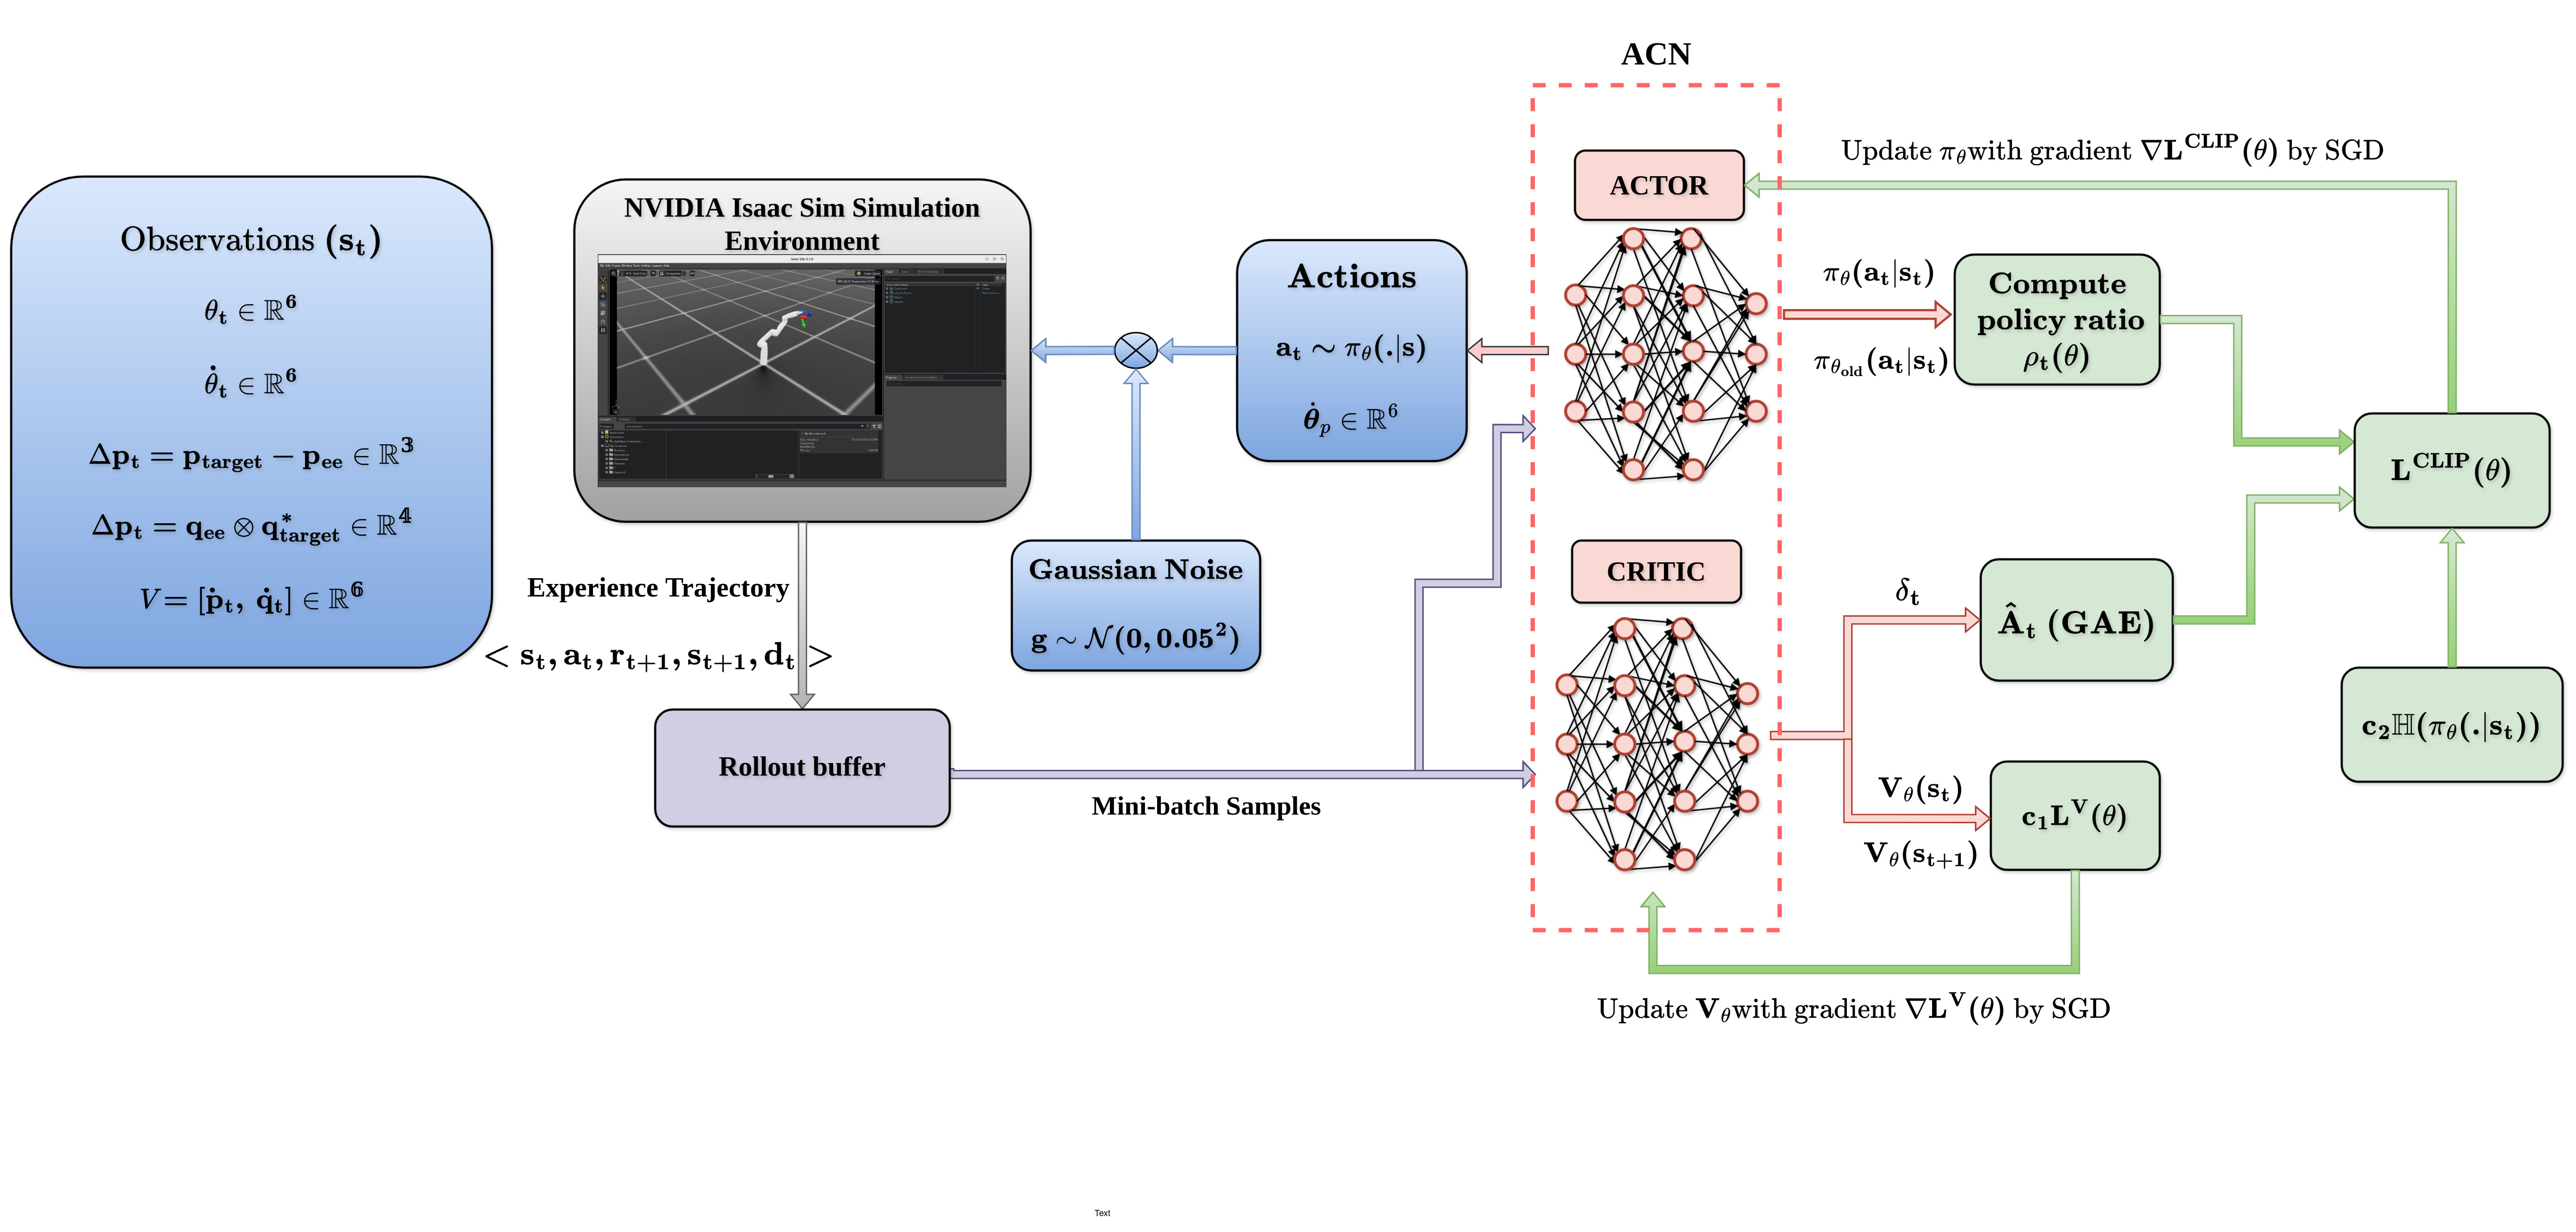
\includegraphics[width=\linewidth]{Images/dikppo/overall_method.jpg}
\caption{Overall method for differential inverse kinematics for trajectory tracking, from the
NVIDIA Isaac Sim environment through the actor-critic network to the PPO policy
update~\citep{sk2025diktracking}.}
\label{fig:dikppo_overall}
\end{figure}

%% ============================================================
\section{Simulation Environment and Reachable-Pose Dataset}\label{sec:dikppo_env}
%% ============================================================

Training is conducted in NVIDIA Isaac Lab with a physics timestep of $\Delta t = 1/120$\,s and a
control decimation of 2, giving a policy frequency of 60\,Hz. The Kinova Gen3 Lite is modelled as a
USD asset with self-collisions enabled, joints are velocity-controlled so the policy output maps
directly to a joint command, and each episode spans 600 steps with the arm initialized to its home
configuration at every reset.

The target poses used for episode initialization are not sampled online but constructed once,
offline, as a fixed dataset: each of the six joints is swept independently across its mechanical
limit range at $5^\circ$ increments, the full combinatorial set of joint-angle tuples is mapped to
its corresponding end-effector pose via forward kinematics, and Isaac Sim's contact-sensing
pipeline discards any configuration that produces self-collision. This procedure yields 1.5 million
collision-free, kinematically valid reachable poses, generated once and reused unchanged across the
full training run. At every episode reset, a target pose is drawn uniformly at random from this
fixed set, and the corresponding pose error, $\Delta \mathbf{p}_t$ and $\Delta \mathbf{Q}_t$ in
Table~\ref{tab:dikppo_obsspace}, is computed relative to the robot's current end-effector pose.
Stochasticity is introduced not by perturbing the target set itself but at the policy output, via
the additive Gaussian action noise developed in Section~\ref{sec:dikppo_ppo}, which is what serves
as the domain-randomization mechanism for sim-to-real transfer. Training runs on a single NVIDIA
GeForce RTX 5060 Ti (16\,GB VRAM); the resulting hyperparameters are collected in
Table~\ref{tab:dikppo_hyper}.

\begin{table}[htbp]
\centering
\caption{PPO hyperparameters for the coupled-reward controller~\citep{sk2025diktracking}.}
\label{tab:dikppo_hyper}
\begin{tabular}{lc}
\toprule
\textbf{Hyperparameter} & \textbf{Value} \\
\midrule
Total timesteps            & $5 \times 10^8$ \\
Parallel environments      & 4096 \\
Steps per rollout ($N_{\text{steps}}$) & 16 \\
Minibatch size              & 4096 \\
Epochs                      & 10 \\
Discount factor ($\gamma$)  & 0.99 \\
GAE parameter ($\lambda$)   & 0.95 \\
Learning rate                & $5 \times 10^{-5}$ \\
Clip range ($\epsilon$)      & 0.13 \\
Entropy coefficient ($c_2$)  & 0.01 \\
Value coefficient ($c_1$)    & 0.5 \\
Network architecture         & $[256 \times 256]$ \\
Activation function           & Tanh \\
Weight initialization          & Orthogonal \\
\bottomrule
\end{tabular}
\end{table}

%% ============================================================
\section{Policy Optimization}\label{sec:dikppo_ppo}
%% ============================================================

At each training iteration, experience tuples $\langle \mathbf{s}_t, \mathbf{a}_t, r_{t+1},
\mathbf{s}_{t+1}, d_t \rangle$ are collected across all 4096 parallel environments over
$N_{\text{steps}} = 16$ steps, yielding 65{,}536 transitions per rollout. Additive Gaussian action
noise is injected at the environment interface before command execution, both to improve robustness
to real actuator imprecision and to serve as implicit domain randomization narrowing the
sim-to-real gap:
\begin{equation}
\mathbf{a}_t = \operatorname{clip}\left( \pi_\theta(\cdot \mid \mathbf{s}_t) + \mathbf{g},\, -1,\, 1 \right),
\qquad \mathbf{g} \sim \mathcal{N}(0,\, 0.05^2 \mathbf{I}_6).
\label{eq:dikppo_actionnoise}
\end{equation}
Advantage estimates use Generalized Advantage Estimation with the critic value $V_\theta(\mathbf{s}_t)$:
\begin{equation}
\hat{A}_t = \sum_{l=0}^{N_{\text{steps}}} (\gamma \lambda)^l\, \delta_{t+l}, \qquad
\delta_t = r_t + \gamma V_\theta(\mathbf{s}_{t+1}) - V_\theta(\mathbf{s}_t),
\label{eq:dikppo_gae}
\end{equation}
and the actor is updated by maximizing the standard clipped PPO objective,
\begin{equation}
L(\theta) = L^{\text{CLIP}}(\theta) - c_1 L^V(\theta) + c_2\, \mathbb{H}\!\left( \pi_\theta(\cdot \mid \mathbf{s}_t) \right),
\label{eq:dikppo_ppoloss}
\end{equation}
where $L^{\text{CLIP}}(\theta) = \mathbb{E}_t\!\left[ \min\!\left( \rho_t(\theta) \hat{A}_t,\,
\operatorname{clip}(\rho_t(\theta), 1-\epsilon, 1+\epsilon)\, \hat{A}_t \right) \right]$ with policy
ratio $\rho_t(\theta) = \pi_\theta(\mathbf{a}_t \mid \mathbf{s}_t) /
\pi_{\theta_{\text{old}}}(\mathbf{a}_t \mid \mathbf{s}_t)$, and $L^V(\theta)$ the mean-squared error
between predicted and target value. Both networks update jointly over 10 epochs per rollout by
minibatch stochastic gradient descent. What distinguishes this controller from a generic PPO
application to trajectory tracking, and what Section~\ref{sec:dikppo_reward} presents as its core
contribution, is the reward this policy is optimizing.

%% ============================================================
\section{Coupled Reward Design}\label{sec:dikppo_reward}
%% ============================================================

Designing a reward for trajectory tracking on a non-spherical wrist requires a careful balance
between position and orientation error convergence: an unconstrained algebraic combination of the
two is susceptible to reward exploitation, where the agent maximizes one objective while leaving
the other under-optimized. The reward function proposed here couples the two through a
min-operator, adds a progress term that explicitly penalizes stagnation, and adds an energy penalty
that suppresses velocity discontinuities, three components combined without manual inter-objective
weighting or staged training curricula. This coupled construction, rather than the choice of PPO as
the underlying optimizer, is the central contribution of this study.

%% ------------------------------------------------------------
\subsection{Pose Reward}\label{subsec:dikppo_pose}
%% ------------------------------------------------------------

Position and orientation errors are first normalized to a common scale so that neither dominates
the other by virtue of its units:
\begin{equation}
e_p = \frac{\lVert \mathbf{p}_{\text{target}} - \mathbf{p}_{ee} \rVert_2}{d_{\max}}, \qquad
e_o = \frac{2 \cos^{-1}\!\left( \left| \operatorname{Re}(\mathbf{Q}_{ee} \otimes \mathbf{Q}_{\text{target}}^*) \right| \right)}{\pi},
\label{eq:dikppo_normerror}
\end{equation}
where $d_{\max}$ is the diagonal of the workspace. Each normalized error is shaped through a
combined inverse-quadratic and logarithmic term,
\begin{equation}
r(x) = \frac{2.5}{1 + 100 x^2} - 0.1 \log\!\left( x + 1 \times 10^{-8} \right),
\label{eq:dikppo_shaping}
\end{equation}
which provides strong attraction near the goal through its inverse-quadratic component while the
logarithmic term maintains a non-zero gradient far from the goal, avoiding the sparse-reward regime
a purely inverse-quadratic shaping would fall into at large error. The two shaped errors are then
coupled by a minimum operator,
\begin{equation}
r_{\text{pose}} = \min\!\left( r(e_p),\, r(e_o) \right),
\label{eq:dikppo_minop}
\end{equation}
so that the reward tracks whichever of position or orientation is currently worse, giving the agent
no incentive to over-optimize the easier objective while neglecting the other, which is precisely
the exploitation an unconstrained sum admits.

%% ------------------------------------------------------------
\subsection{Progress Reward}\label{subsec:dikppo_progress}
%% ------------------------------------------------------------

The pose reward shapes the magnitude of the error but gives no explicit incentive to reduce it at
every timestep; a policy could sustain a moderate, unchanging error indefinitely and still collect a
non-trivial reward. The per-step change in each error component is
\begin{equation}
\Delta e_p = e_{p,t} - e_{p,t-1}, \qquad \Delta e_o = e_{o,t} - e_{o,t-1},
\label{eq:dikppo_delta}
\end{equation}
with a negative value indicating improvement. Rather than rewarding progress on both dimensions
simultaneously, the progress reward is applied only to the dominant error, the dimension currently
making the least progress:
\begin{equation}
\Delta e =
\begin{cases}
\Delta e_p, & \Delta e_p \geq \Delta e_o, \\
\Delta e_o, & \Delta e_p < \Delta e_o,
\end{cases}
\label{eq:dikppo_dominant}
\end{equation}
and shaped asymmetrically so that improvement and regression are not penalized symmetrically:
\begin{equation}
r_{\text{prog}}(\Delta e) =
\begin{cases}
4(-\Delta e + 0.25)^{0.5} - 2, & \Delta e < 0, \\
-2 \exp(2 \Delta e) + 2, & \Delta e \geq 0.
\end{cases}
\label{eq:dikppo_progress}
\end{equation}
Both branches are offset to avoid a discontinuous reward cliff at $\Delta e = 0$, which would
otherwise destabilize value estimation. The square-root shaping on improvement provides diminishing
returns for large progress steps, discouraging aggressive overshoot, while the exponential penalty
for regression imposes a sharply increasing cost as error grows, creating steady pressure toward
monotonic convergence.

%% ------------------------------------------------------------
\subsection{Energy Penalty and Total Reward}\label{subsec:dikppo_energy}
%% ------------------------------------------------------------

Trajectory tracking further requires smooth, continuous joint motion throughout, not merely
accurate terminal poses. A continuous energy penalty on joint velocity commands is applied at every
timestep,
\begin{equation}
r_{\text{energy}} = 1 - \exp\!\left( 0.2 \sum_{i=1}^{6} \dot{q}_i^2 \right),
\label{eq:dikppo_energy}
\end{equation}
whose exponential form imposes a sharply increasing cost as aggregate joint velocity grows. The
total reward at each timestep is the sum of the three components,
\begin{equation}
r_{t+1} = r_{\text{pose}} + r_{\text{prog}} + r_{\text{energy}},
\label{eq:dikppo_totalreward}
\end{equation}
combining accurate pose convergence, per-step progress pressure on whichever error is worst, and
smooth, hardware-safe velocity commands, without any of the three components requiring separate
tuning against the others.

%% ============================================================
\section{Sim-to-Real Transfer}\label{sec:dikppo_sim2real}
%% ============================================================

At deployment, the policy output is clipped and converted from normalized radians to the degrees
per second the Kinova Kortex API~\citep{Kinovarobotics_2025} requires:
\begin{equation}
\dot{\mathbf{q}}_p = \operatorname{clip}(\mathbf{a}_t,\, -1,\, 1) \cdot \frac{180}{\pi} \;\; (^\circ/\text{s}),
\label{eq:dikppo_hwvel}
\end{equation}
with observation parity maintained directly from Kortex actuator feedback, preserving the exact
19-dimensional structure seen during training (Figure~\ref{fig:dikppo_sim2real}).

\begin{figure}[htbp]
\centering
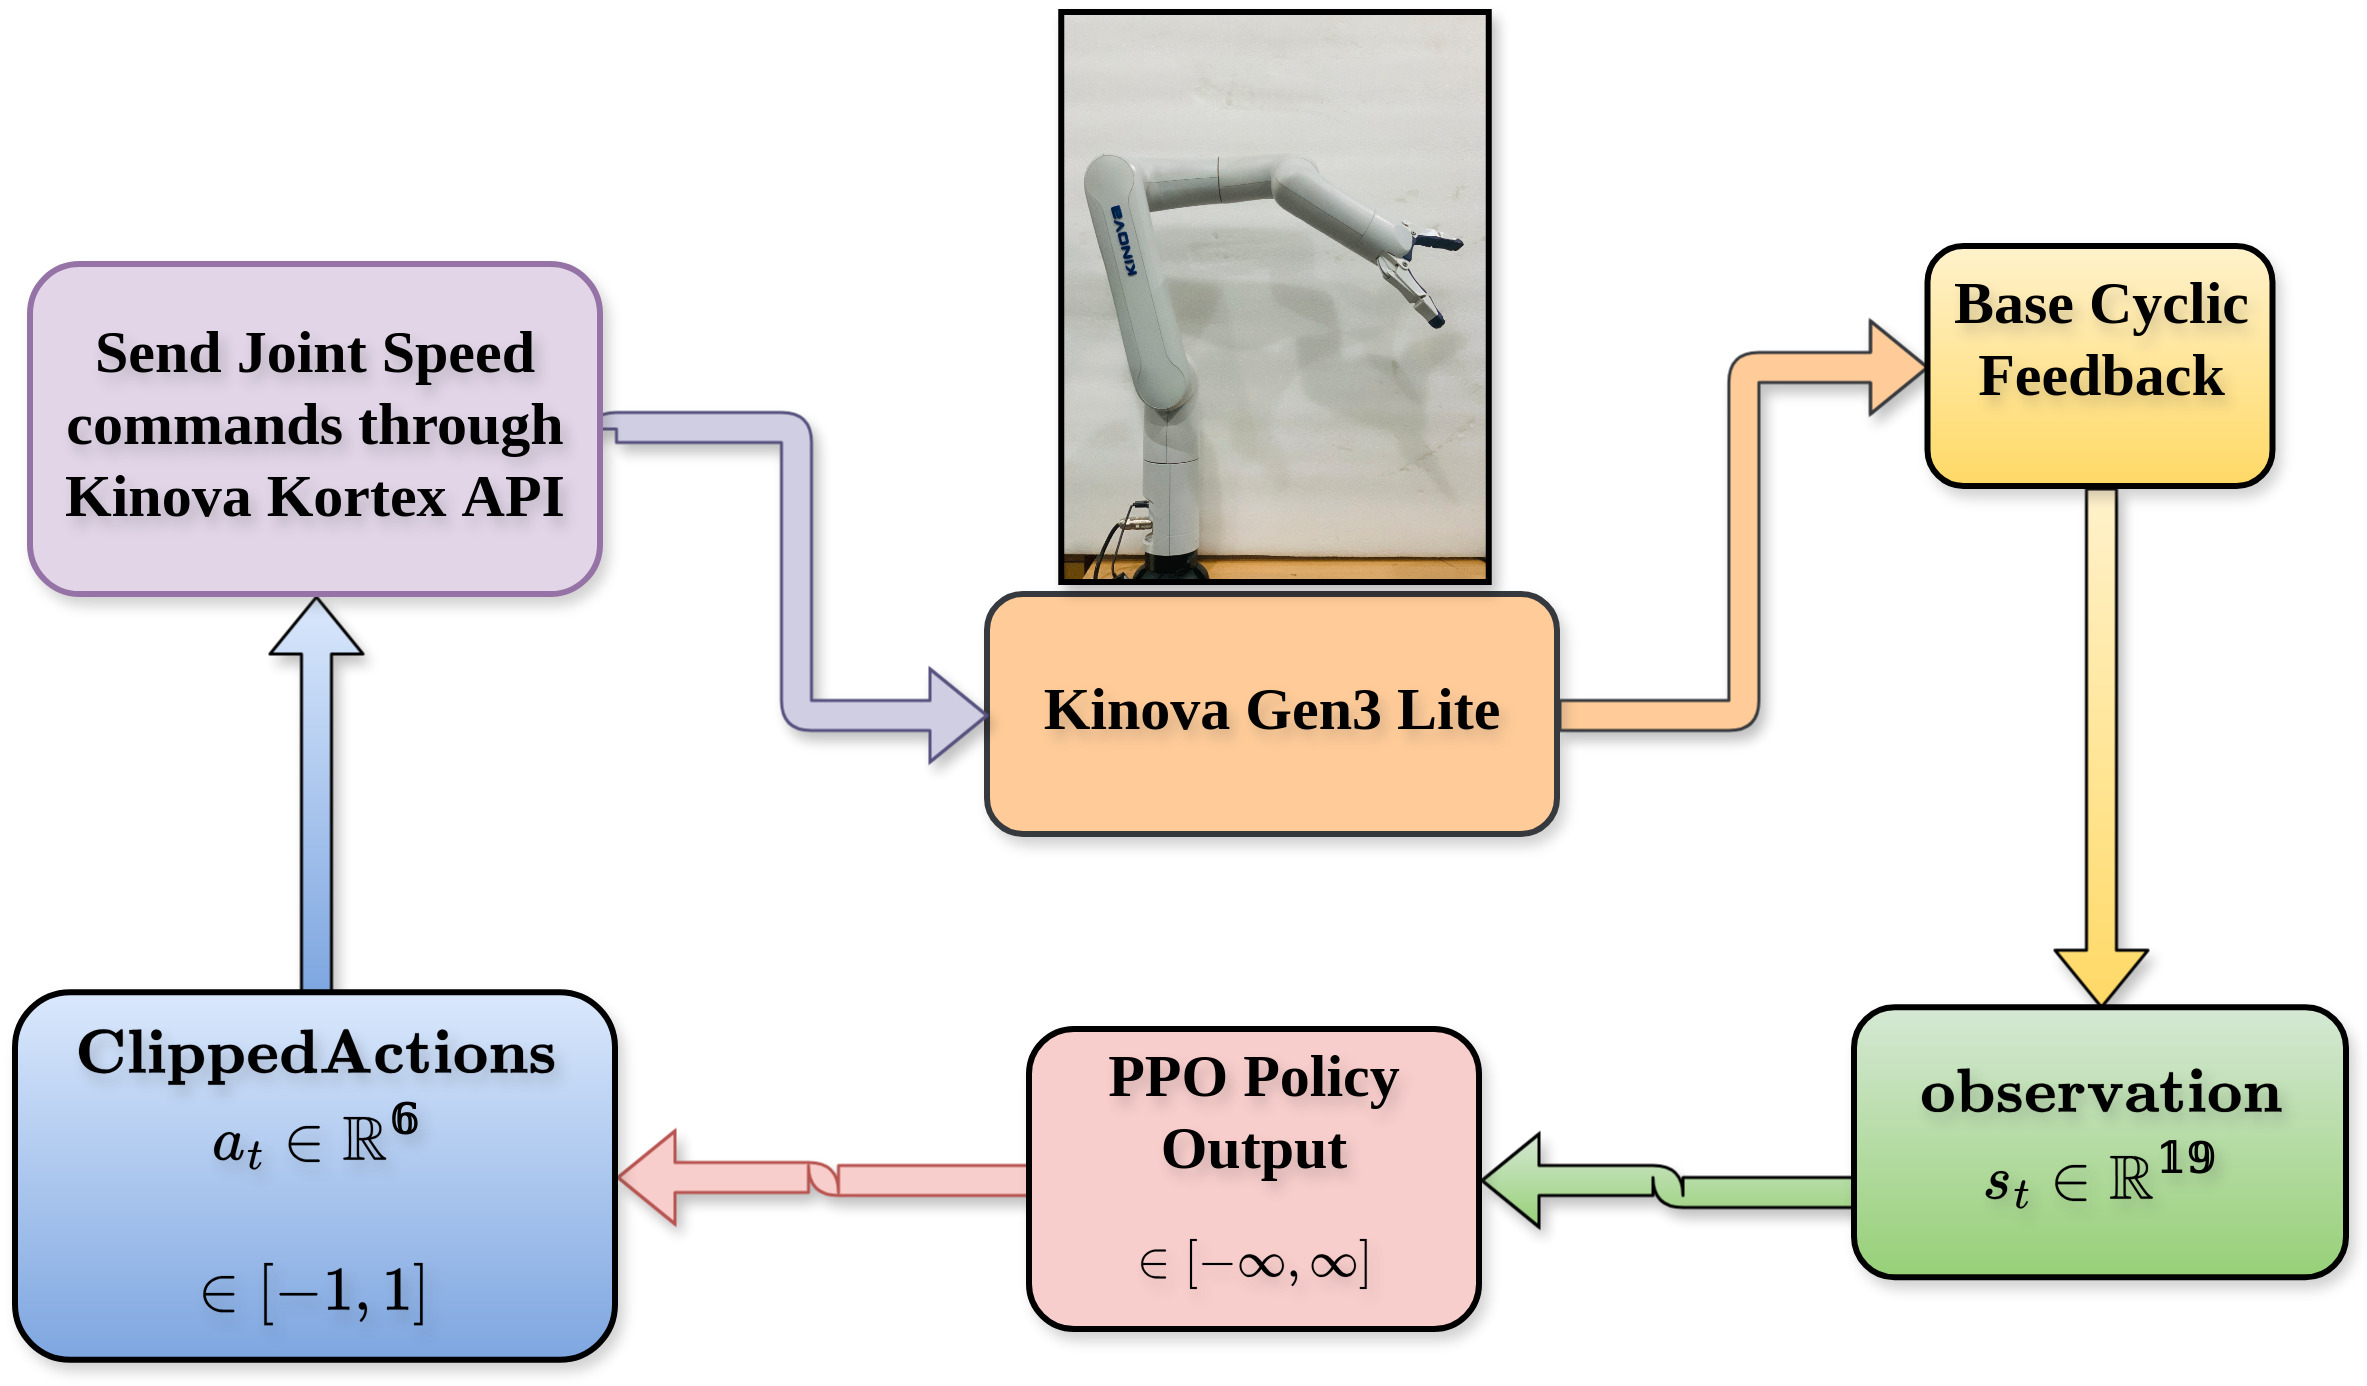
\includegraphics[width=0.75\linewidth]{Images/dikppo/sim_to_real_architecture.jpg}
\caption{Sim-to-real architecture: policy observation, PPO output, action clipping, and dispatch to
the Kinova Gen3 Lite via the Kortex API~\citep{sk2025diktracking}.}
\label{fig:dikppo_sim2real}
\end{figure}

The policy is deployed on an Intel NUC9 Extreme (16-core CPU, 32\,GB RAM), reaching inference at
approximately 1.3\,kHz, while the Kinova Kortex API imposes an effective closed-loop control
frequency of 20\,Hz since feedback reading and command dispatch execute sequentially. This is
roughly one third of the 60\,Hz frequency used during training; because the policy is a memoryless
mapping from instantaneous observation to velocity command, with no recurrent state, a lower
deployment frequency only extends the zero-order-hold duration of each command rather than
invalidating any individual policy input. Consistent with the action noise of
Equation~\eqref{eq:dikppo_actionnoise} and the energy penalty of Equation~\eqref{eq:dikppo_energy}
jointly bounding output velocity magnitude, no frequency-related degradation was observed at the
tested trajectory speed: hardware position RMSE on the circular trajectory (6.3\,mm) was in fact
lower than the simulation RMSE (9.95\,mm), consistent with actuator damping and low-level velocity
smoothing further attenuating the discretized commands at the tested speed, though this should be
read as evidence against degradation at that specific speed rather than general frequency
invariance.

%% ============================================================
\section{Baseline Comparison and Reward Ablation}\label{sec:dikppo_ablation}
%% ============================================================

Two questions are separated deliberately in validating this controller: whether the reward
structure or the choice of PPO as the optimizing algorithm is responsible for the result, and which
of the reward's three components is doing the work. Section~\ref{subsec:dikppo_algcompare}
addresses the first by holding the reward fixed and varying the algorithm; Section
\ref{subsec:dikppo_rewardablation} addresses the second by holding PPO fixed and varying the
reward.

%% ------------------------------------------------------------
\subsection{Algorithm Comparison}\label{subsec:dikppo_algcompare}
%% ------------------------------------------------------------

The proposed coupled reward, Equation~\eqref{eq:dikppo_totalreward}, is paired with TRPO and with
SAC under an otherwise identical setup, alongside sparse-reward variants (terminal success only) of
PPO and SAC, to isolate whether the reward or the algorithm drives the result.

\begin{figure}[htbp]
\centering
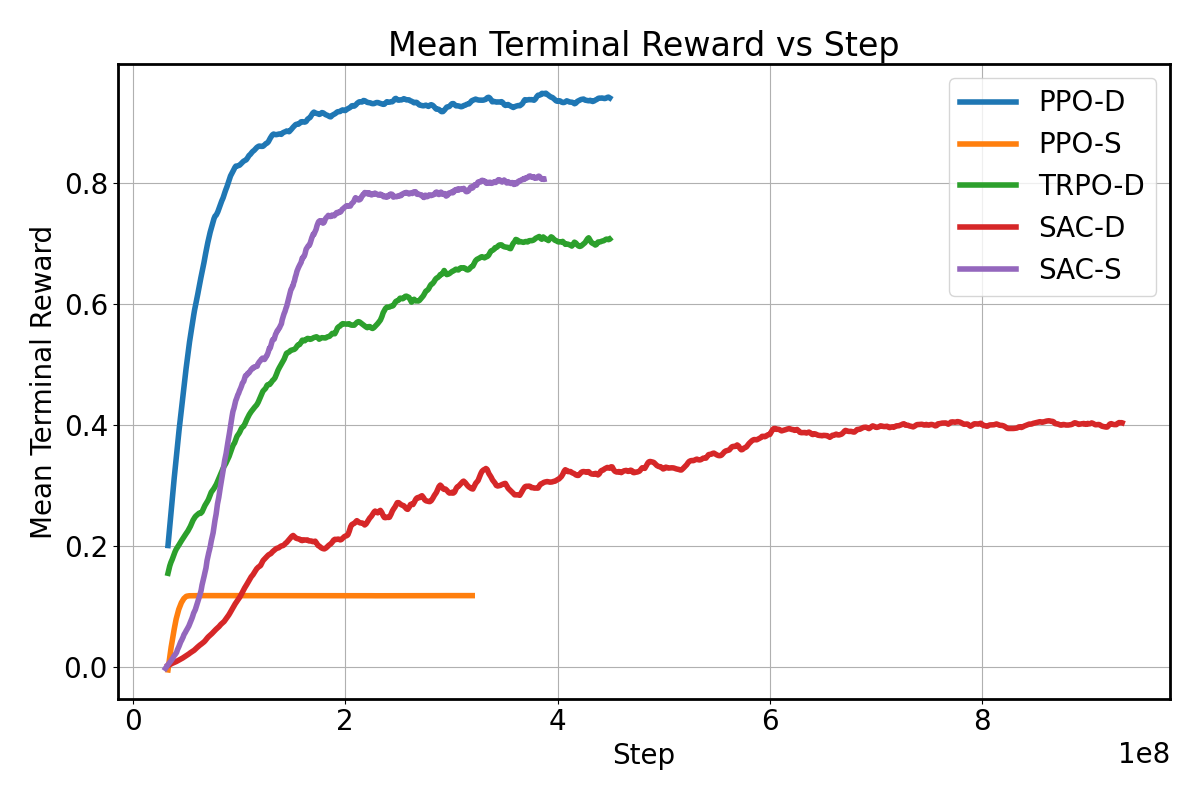
\includegraphics[width=0.7\linewidth]{Images/dikppo/training_curves.png}
\caption{Mean terminal reward versus training step for PPO with the dense coupled reward (PPO-D),
PPO with a sparse reward (PPO-S), TRPO with the dense reward (TRPO-D), and SAC with dense and
sparse rewards (SAC-D, SAC-S)~\citep{sk2025diktracking}.}
\label{fig:dikppo_traincurves}
\end{figure}

Figure~\ref{fig:dikppo_traincurves} shows PPO-D converging monotonically to a mean terminal reward
of $\approx 0.93$, the highest and smoothest of any configuration. TRPO-D, despite sharing the
identical coupled reward and PPO's conservative trust-region philosophy, converges more slowly and
plateaus at $\approx 0.71$: its exact KL-divergence constraint, versus PPO's clipped surrogate
approximation, requires a more expensive constrained update per step, and under an identical
timestep budget this leaves TRPO less converged. SAC exhibits the opposite failure mode: SAC's
maximum-entropy objective, which explicitly rewards maintaining stochasticity in the action
distribution, directly conflicts with the exponential energy penalty of
Equation~\eqref{eq:dikppo_energy}, which penalizes any non-zero joint velocity near convergence. The
two objectives settle into a stable compromise in which the policy sustains a small, persistent
non-zero error rather than fully converging, visible as SAC-D and SAC-S plateauing at $\approx 0.40$
and $\approx 0.81$ respectively; notably SAC-D, trained for nearly double SAC-S's step budget in
the hope that additional experience would let the dense reward eventually dominate, remains well
below SAC-S, indicating the entropy-energy conflict is not resolved by additional training. PPO-S
stagnates almost immediately at $\approx 0.12$, confirming that without the dense, coupled reward
shaping of Section~\ref{sec:dikppo_reward}, sparse terminal feedback alone is too infrequent for
the policy to learn the precise joint coordination continuous trajectory tracking requires. Training
wall-clock cost varies substantially with these dynamics, from PPO-D's 1\,h 5\,m to TRPO-D's 3\,h
14\,m for the same step count, so the proposed method's accuracy and smoothness gains come at a
one-time, sub-two-hour training cost rather than any added cost per deployment.

%% ------------------------------------------------------------
\subsection{Reward Component Ablation}\label{subsec:dikppo_rewardablation}
%% ------------------------------------------------------------

Holding PPO fixed, four reward variants isolate the contribution of each component on circular
trajectory tracking: (a) a conventional (unshaped, uncoupled) reward, (b) the min-operator pose
reward plus progress shaping without the energy penalty, (c) the min-operator pose reward plus the
energy penalty without progress shaping, and (d) the full reward of
Equation~\eqref{eq:dikppo_totalreward}.

\begin{figure}[htbp]
\centering
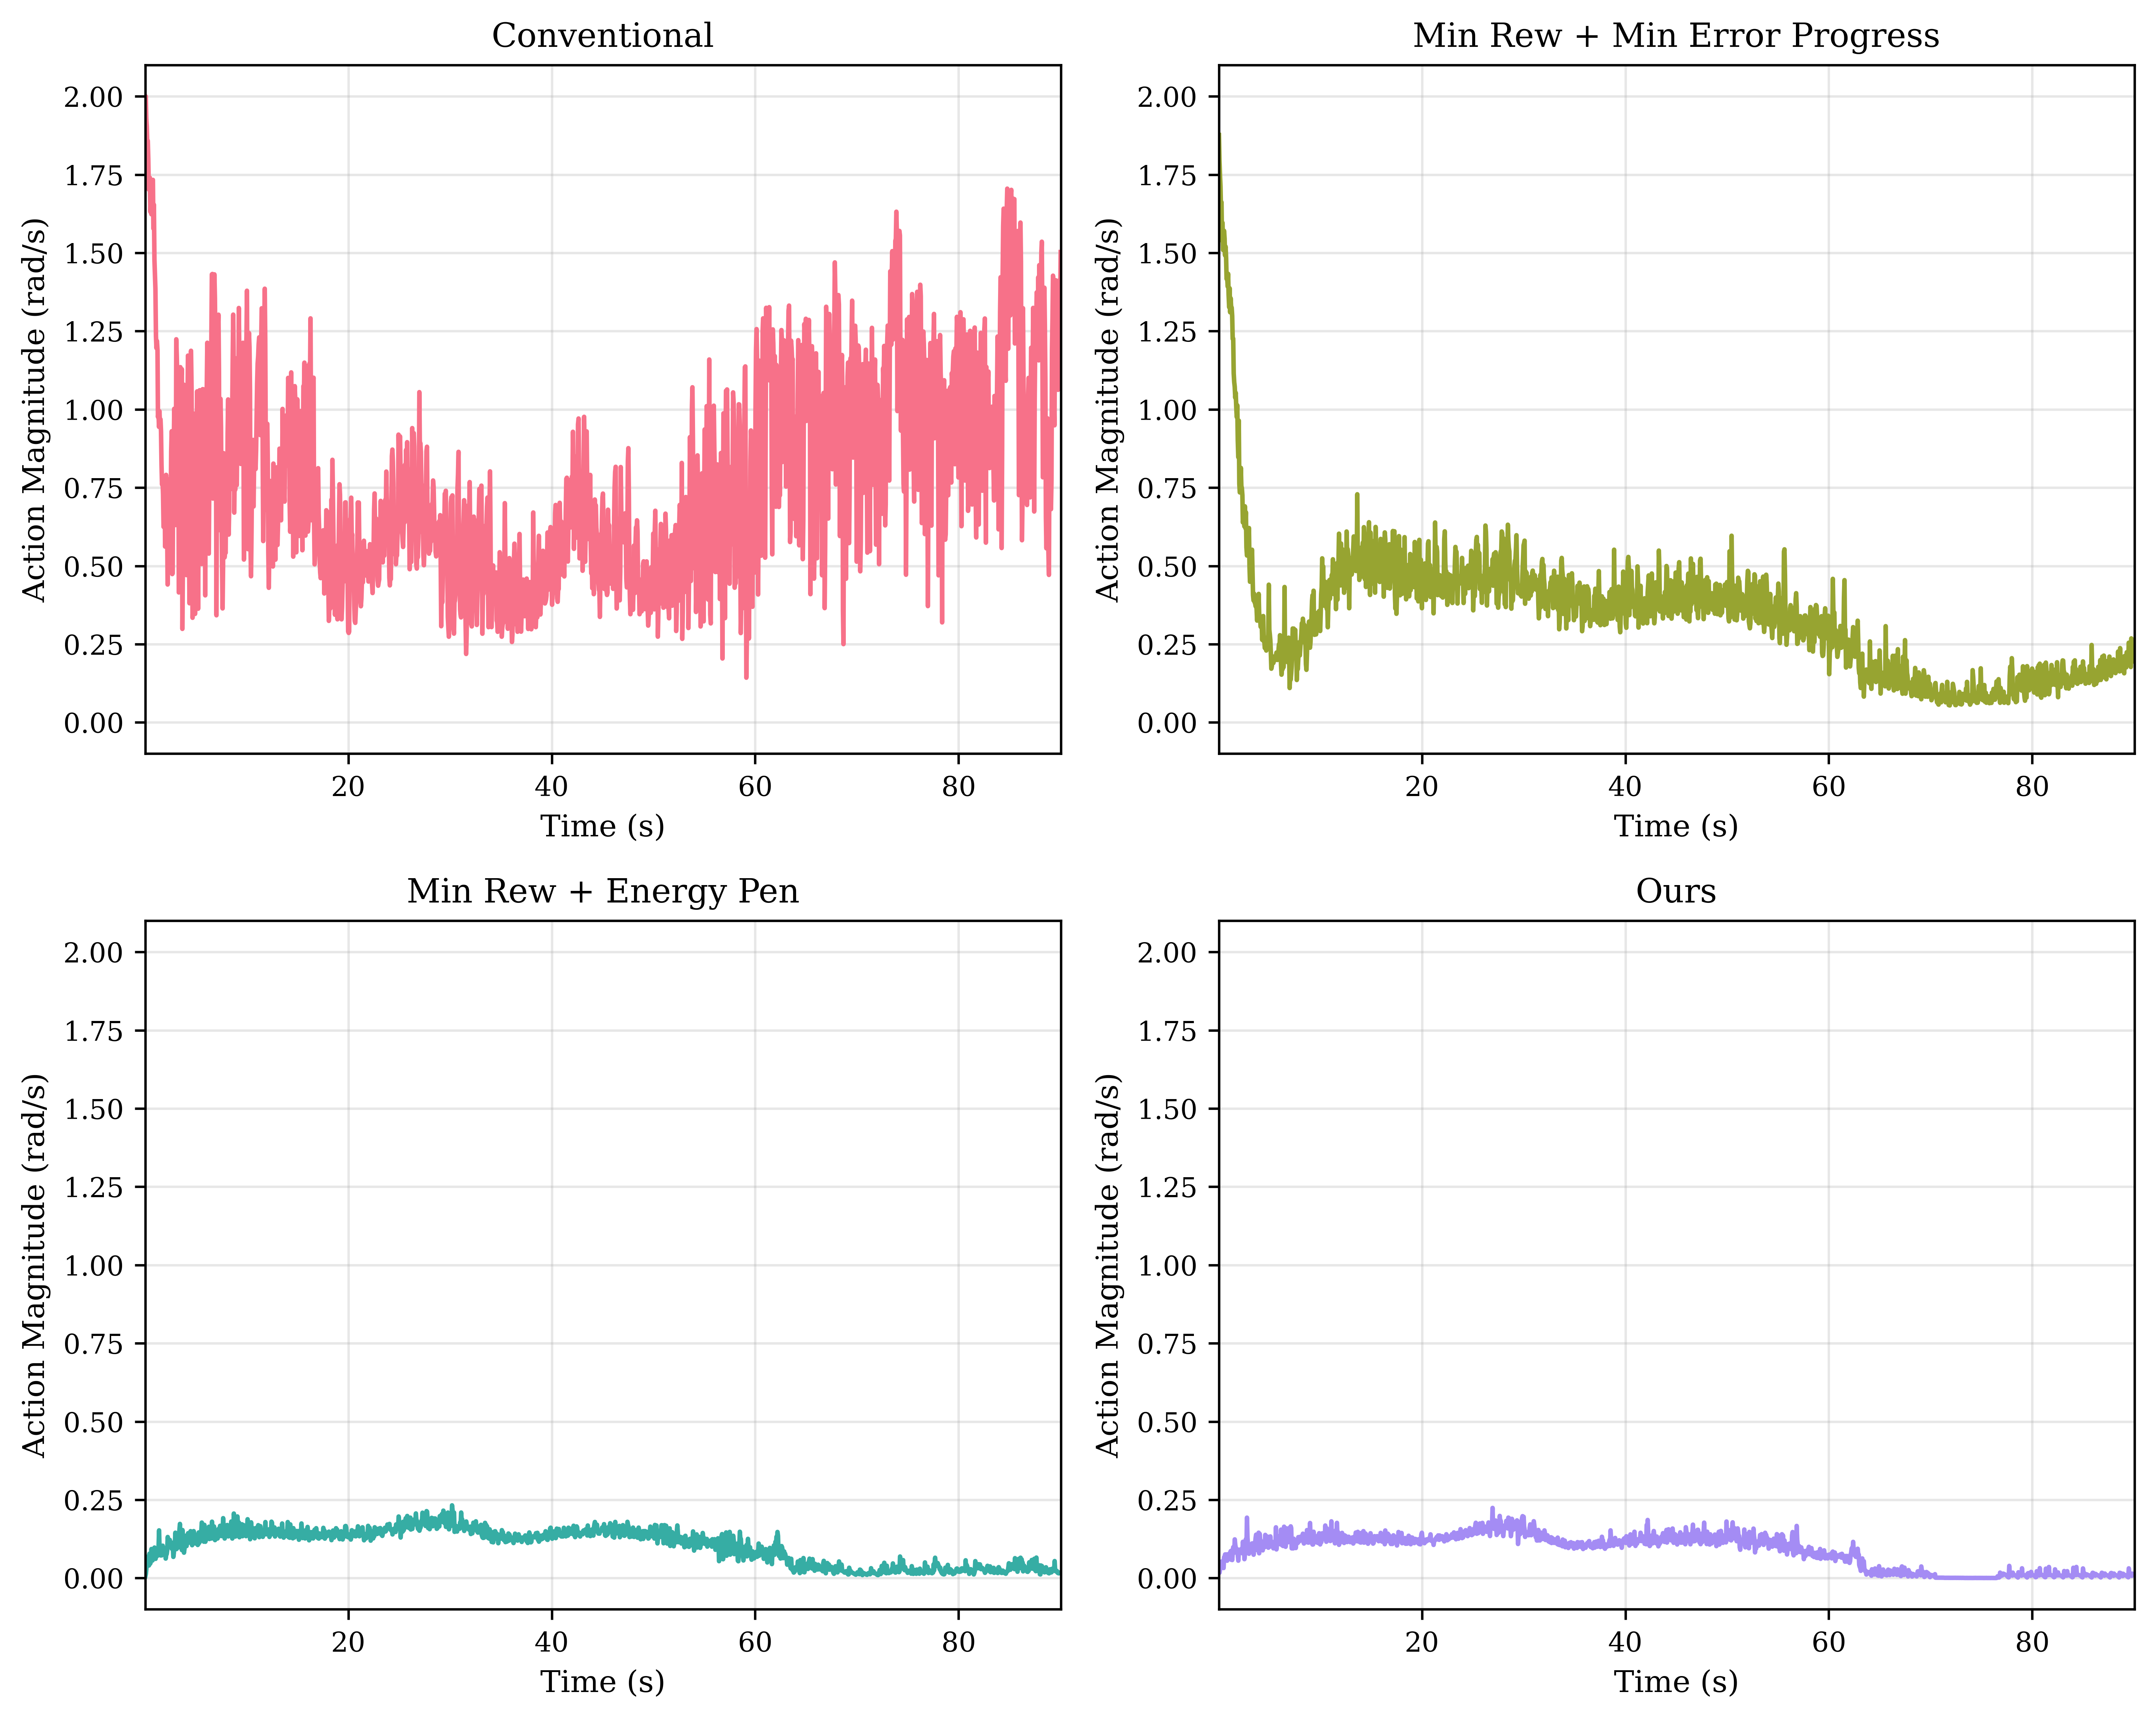
\includegraphics[width=0.85\linewidth]{Images/dikppo/ablation_joint_velocity.png}
\caption{Joint velocity command magnitude across the four reward ablation variants during circular
trajectory tracking~\citep{sk2025diktracking}.}
\label{fig:dikppo_ablationvel}
\end{figure}

\begin{figure}[htbp]
\centering
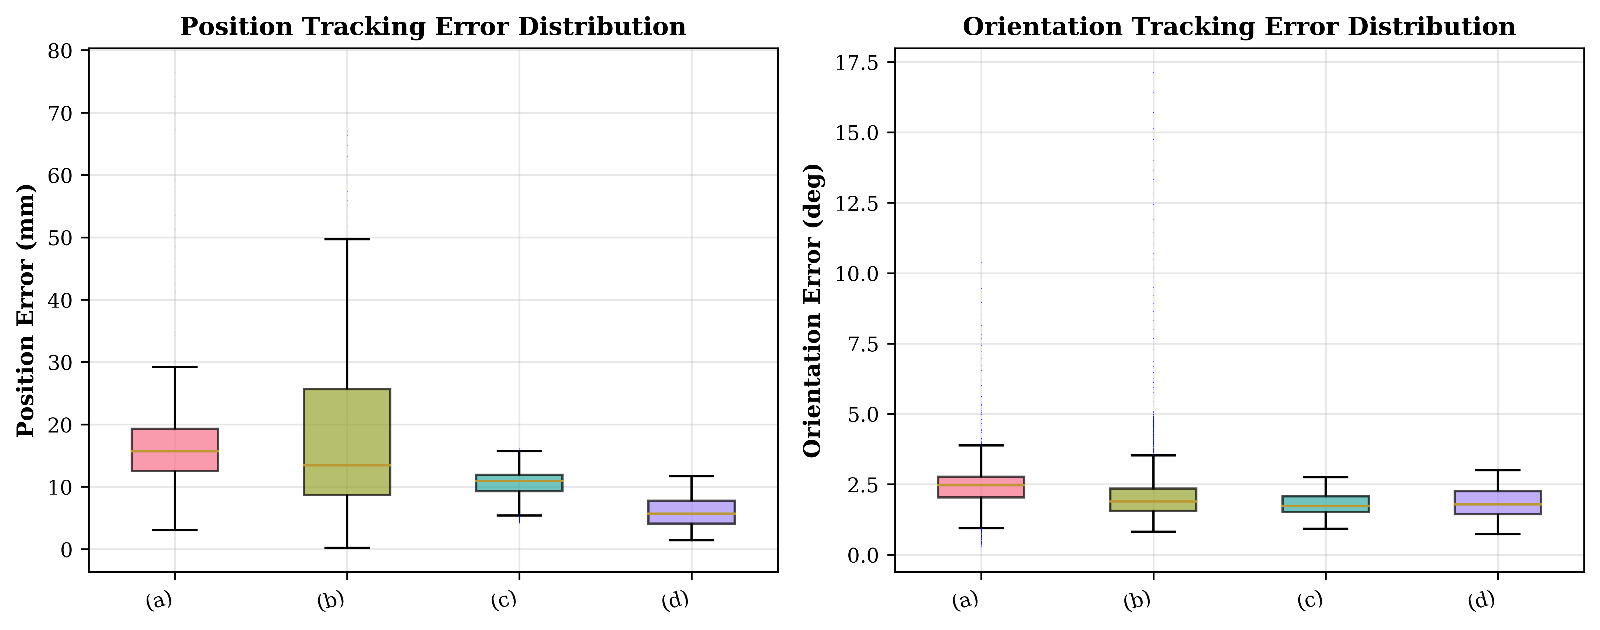
\includegraphics[width=0.85\linewidth]{Images/dikppo/ablation_error_boxplot.jpeg}
\caption{Position and orientation tracking error distribution across the four reward ablation
variants~\citep{sk2025diktracking}.}
\label{fig:dikppo_ablationerr}
\end{figure}

\begin{figure}[htbp]
\centering
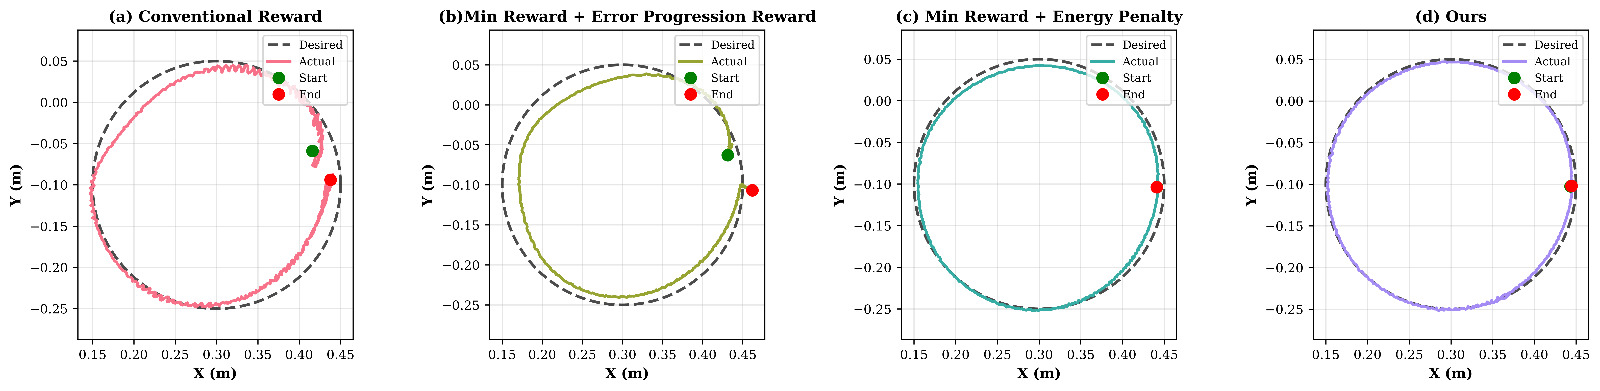
\includegraphics[width=\linewidth]{Images/dikppo/ablation_xy_trajectory.jpeg}
\caption{XY trajectory comparison across the four reward ablation variants on circular tracking:
(a) conventional, (b) min reward plus progress, (c) min reward plus energy penalty, (d) full
reward~\citep{sk2025diktracking}.}
\label{fig:dikppo_ablationtraj}
\end{figure}

Figure~\ref{fig:dikppo_ablationvel} shows the energy penalty's direct effect: peak action magnitude
falls from 2.0\,rad/s under the conventional reward to below 0.25\,rad/s under the full reward,
with variant (b), progress shaping without the energy penalty, still producing large transient
velocity spikes that collapse into erratic oscillation, confirming the energy term rather than the
min-operator is what suppresses these spikes. Figure~\ref{fig:dikppo_ablationerr} shows the
conventional reward (a) maintaining persistent 15 to 20\,mm oscillation that never settles below
threshold, variant (c), the energy penalty without progress shaping, achieving stable sub-threshold
tracking but at a higher steady-state median of 10\,mm, and the full reward (d) achieving the
lowest median position error of 6\,mm with the tightest distribution, consistently tracking below
10\,mm throughout. Figure~\ref{fig:dikppo_ablationtraj} shows the same pattern geometrically: the
conventional reward fails to complete the circular path at all, deviating substantially near the
start; variant (b) completes the circle but with visible radial deviation; variants (c) and (d)
closely follow the desired trajectory, with the full reward (d) achieving near-perfect circular
tracking. Together these confirm that all three reward components, the min-operator pose coupling,
the asymmetric progress shaping, and the energy penalty, are each necessary, and that no pair alone
reproduces the full reward's combination of accuracy and smoothness.

%% ============================================================
\section{Results: Simulation and Hardware Trajectory Tracking}\label{sec:dikppo_results}
%% ============================================================

Final validation compares the trained policy (PPO-D) against five baselines, TRAC-IK, DLS, velocity
QP, TRPO-D, and SAC-S, spanning classical numerical, classical velocity-level, and alternative
learned methods, across three trajectory geometries chosen to span fixed orientation (circle),
periodically varying orientation (lemniscate), and high-curvature multi-axis motion (3-D
Lissajous).

\begin{figure}[htbp]
\centering
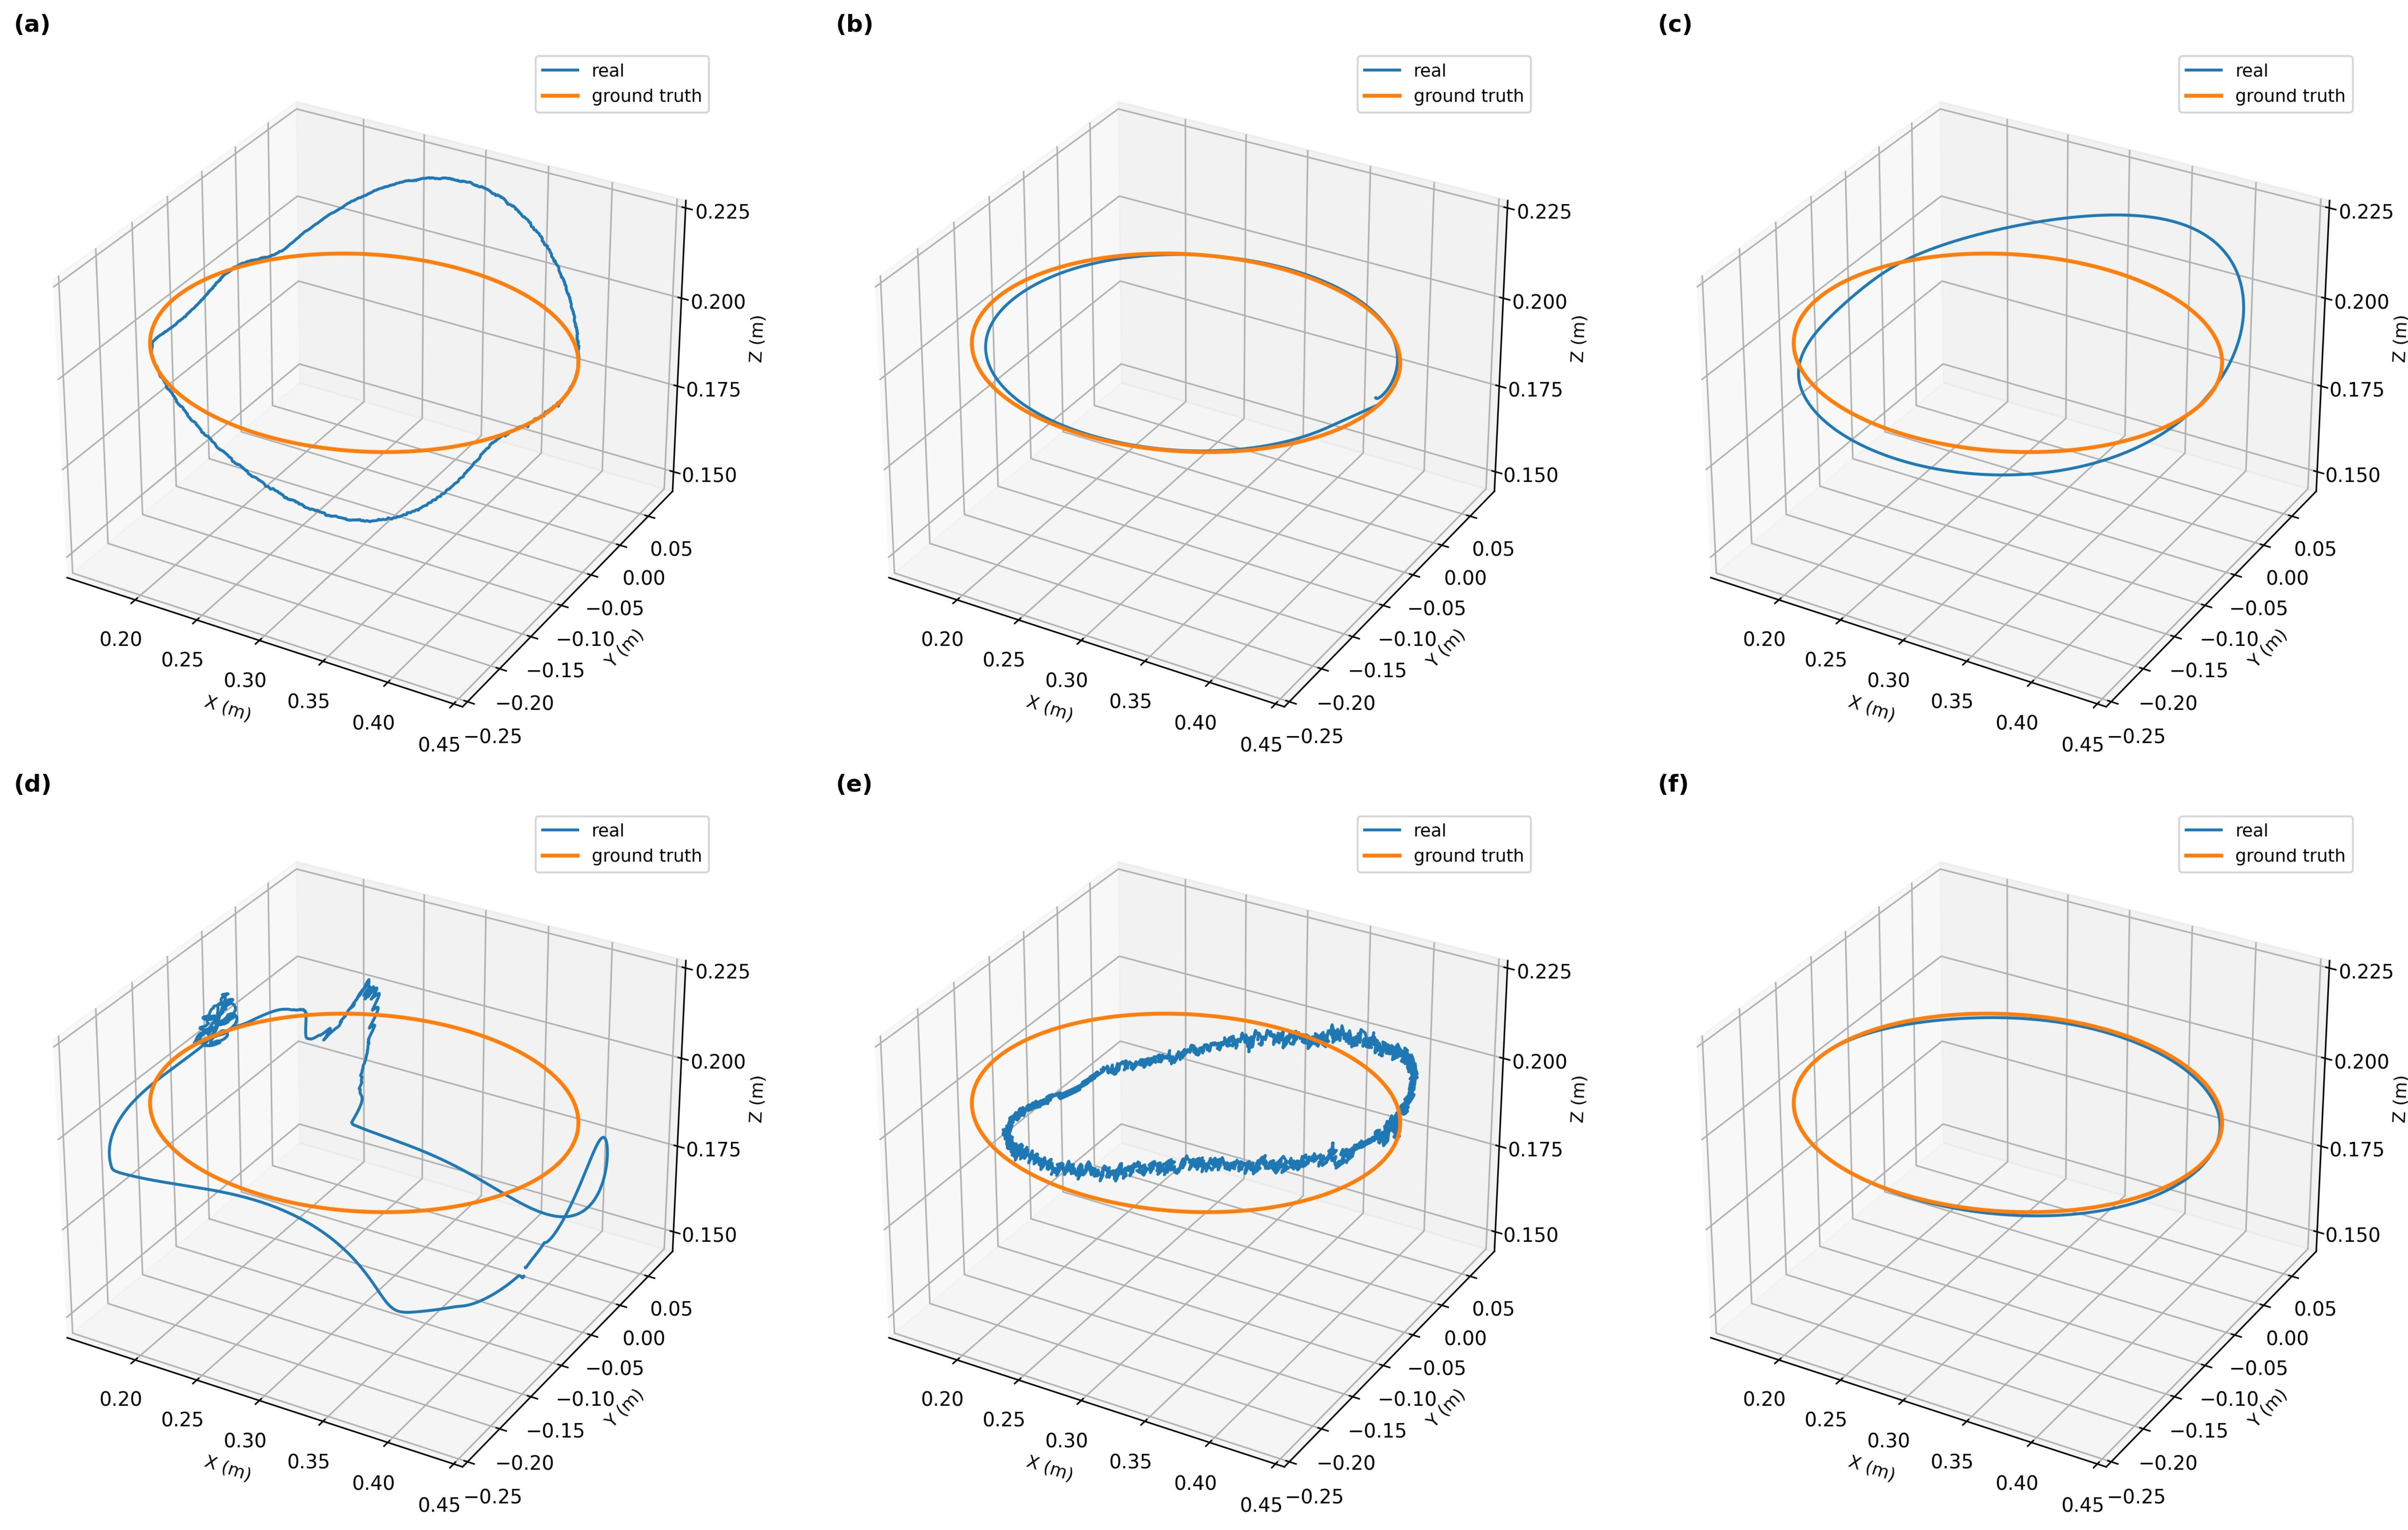
\includegraphics[width=\linewidth]{Images/dikppo/circle_comparison.jpg}
\caption{Circle trajectory comparison: (a) TRAC-IK, (b) DLS pseudo-inverse Jacobian, (c) velocity
QP, (d) TRPO-D, (e) SAC-S, (f) PPO-D~\citep{sk2025diktracking}.}
\label{fig:dikppo_circlecomp}
\end{figure}

\begin{table}[htbp]
\centering
\caption{Simulation performance across circle, lemniscate, and 3-D Lissajous trajectories, with
frozen per-method action scales. No classical baseline is uniformly best; PPO is the only method
with stable accuracy and smoothness across all three geometries. Best value per metric in
bold~\citep{sk2025diktracking}.}
\label{tab:dikppo_simresults}
\begin{tabular}{llccc}
\toprule
\textbf{Method} & \textbf{Curve} & \textbf{Pos. RMSE (m)} & \textbf{Orn. RMSE (rad)} & \textbf{Smoothness} \\
\midrule
\multirow{3}{*}{TRAC-IK} & Circle & 0.001242 & 0.003409 & 54.55 \\
                          & Lemniscate & \textbf{0.001073} & 0.004332 & 52.00 \\
                          & Lissajous & 0.035272 & 0.052286 & 62.16 \\
\midrule
\multirow{3}{*}{DLS}     & Circle & 0.016046 & \textbf{0.000767} & 0.0134 \\
                          & Lemniscate & 0.013554 & 0.036097 & 0.0159 \\
                          & Lissajous & 0.027939 & 0.020683 & 0.0222 \\
\midrule
\multirow{3}{*}{Vel. QP} & Circle & 0.011013 & 0.002900 & 0.0124 \\
                          & Lemniscate & 0.013254 & 0.003857 & 0.0294 \\
                          & Lissajous & 0.035303 & 0.008647 & 0.0164 \\
\midrule
\multirow{3}{*}{TRPO}    & Circle & 0.089448 & 0.372891 & 2.92 \\
                          & Lemniscate & 0.130428 & 0.383532 & 0.141 \\
                          & Lissajous & 0.122329 & 0.257595 & 0.815 \\
\midrule
\multirow{3}{*}{SAC}     & Circle & 0.029320 & 0.051513 & 19.78 \\
                          & Lemniscate & 0.030142 & 0.051104 & 19.08 \\
                          & Lissajous & 0.029181 & 0.050908 & 18.85 \\
\midrule
\multirow{3}{*}{\textbf{PPO}} & Circle & 0.009951 & 0.026476 & \textbf{0.0055} \\
                          & Lemniscate & 0.010650 & 0.023536 & 0.0107 \\
                          & Lissajous & 0.016667 & 0.043686 & 0.0147 \\
\bottomrule
\end{tabular}
\end{table}

Table~\ref{tab:dikppo_simresults} and Figure~\ref{fig:dikppo_circlecomp} show that no single
classical baseline is uniformly competitive, and the pattern of failure for each follows directly
from its underlying mechanism rather than a tuning artefact. TRAC-IK achieves the lowest position
RMSE on the circle (1.2\,mm) and lemniscate (1.07\,mm), since resolving each waypoint as an
independent constrained optimization allows near-exact convergence at every individual pose in a
noiseless simulation, but with no explicit coupling between consecutive solves, small differences in
optimizer convergence translate directly into joint-space discontinuities frame to frame, giving it
a smoothness index three to four orders of magnitude worse than every other method, and on the
Lissajous curve, where curvature and orientation both vary, its nearest-seed assumption breaks down
and position RMSE degrades roughly 30-fold relative to the circle. DLS's fixed-gain
error-coupling strongly favours orientation correction on the circle, where required angular
correction is small, giving the best orientation RMSE of any method there, but the same fixed gain
cannot adaptively reallocate correction authority on the lemniscate, where orientation must vary
continuously, and its orientation RMSE there is worse than PPO's on the identical curve. TRPO shares
PPO's coupled reward and on-policy structure but its exact KL-divergence constraint leaves it less
converged under an identical training budget, producing both higher residual error and
substantially worse smoothness than PPO on every curve. SAC's maximum-entropy objective again
directly conflicts with the energy penalty, producing a persistent radial offset of
$\approx 2.9$\,cm essentially unchanged across all three curves, consistent with an entropy-energy
trade-off rather than a tracking failure specific to any one geometry. PPO does not achieve the
single lowest RMSE on every curve, but it is the only method whose position RMSE stays confined to a
narrow 9.9 to 16.7\,mm band across all three geometries while every classical baseline degrades
sharply on at least one, and it is the smoothest method by one to four orders of magnitude on every
curve, a direct, traceable consequence of the min-operator pose coupling, the asymmetric progress
shaping, and the energy penalty developed in Section~\ref{sec:dikppo_reward}, none of which any
baseline shares.

\begin{figure}[htbp]
\centering
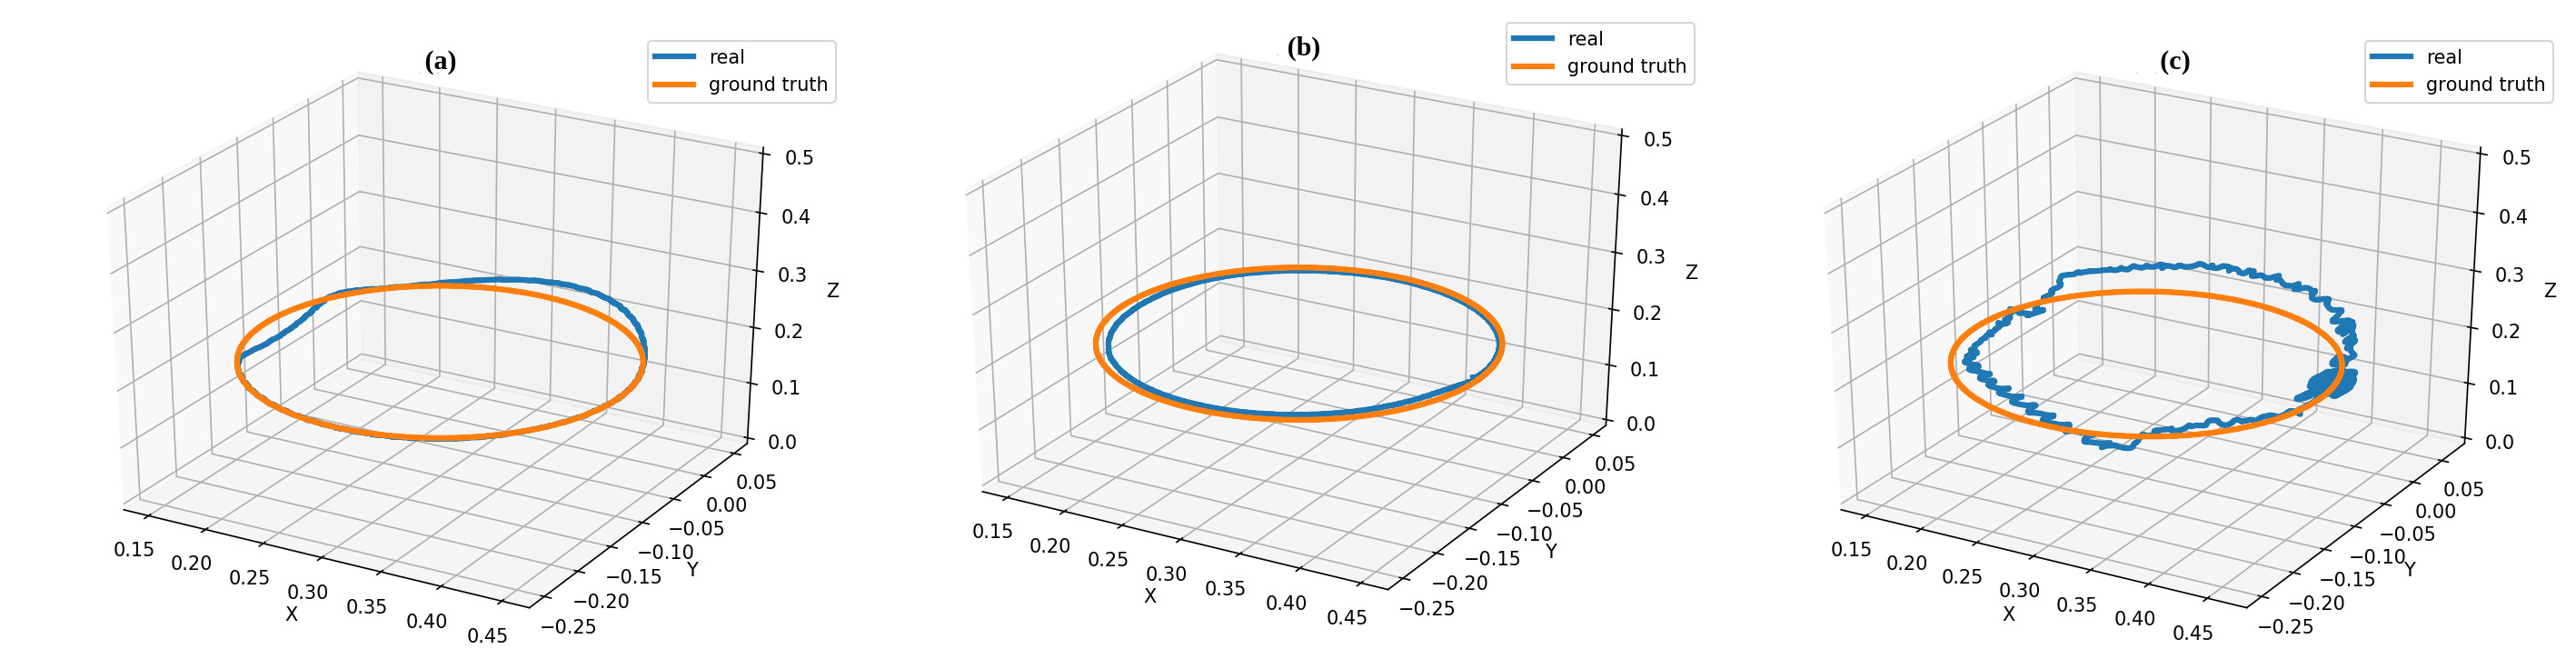
\includegraphics[width=\linewidth]{Images/dikppo/hardware_deployment_baselines.jpg}
\caption{Real-time hardware deployment of (a) TRAC-IK, (b) DLS, and (c) SAC-S on the circular
trajectory~\citep{sk2025diktracking}.}
\label{fig:dikppo_hwbaselines}
\end{figure}

\begin{figure}[htbp]
\centering
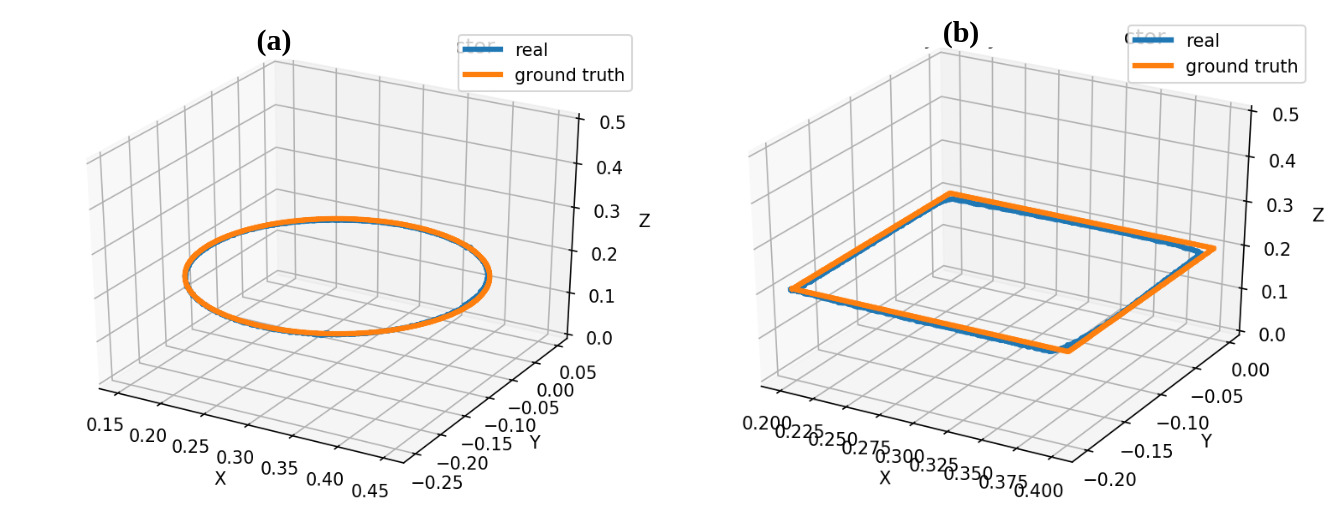
\includegraphics[width=0.85\linewidth]{Images/dikppo/hardware_circle_square.jpg}
\caption{Real-time hardware trajectory tracking of (a) circle and (b) square, both with constant
end-effector orientation~\citep{sk2025diktracking}.}
\label{fig:dikppo_hwcirclesquare}
\end{figure}

\begin{figure}[htbp]
\centering
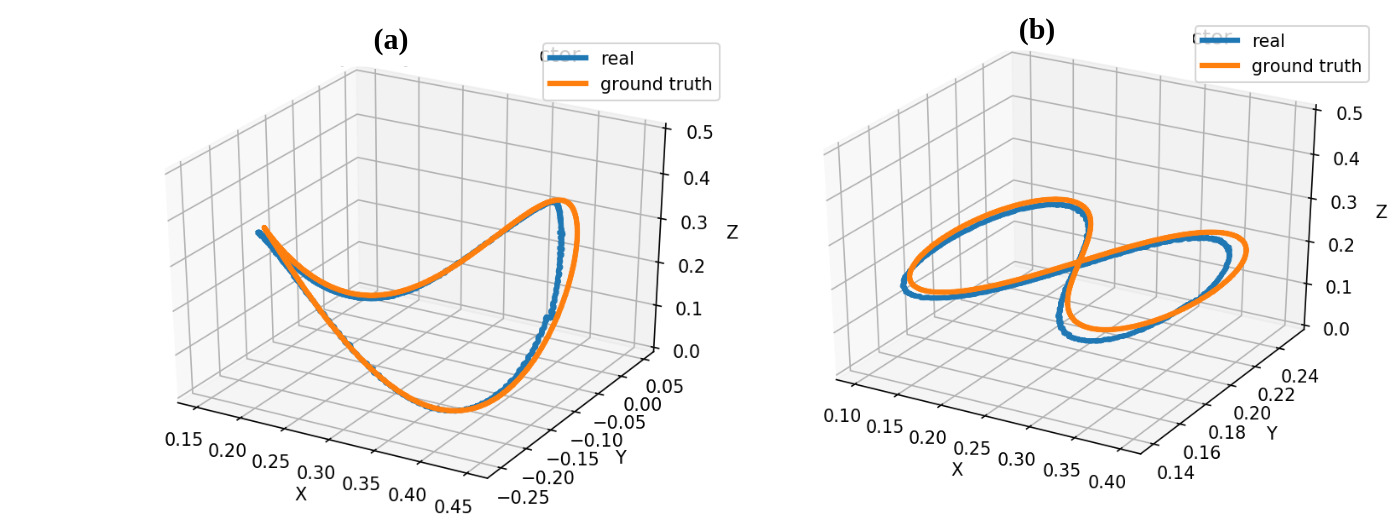
\includegraphics[width=0.85\linewidth]{Images/dikppo/hardware_lissajous_lemniscate.jpg}
\caption{Real-time hardware trajectory tracking of (a) 3-D Lissajous and (b) lemniscate, both with
varying end-effector orientation~\citep{sk2025diktracking}.}
\label{fig:dikppo_hwlissajous}
\end{figure}

\begin{table}[htbp]
\centering
\caption{Hardware performance on the Kinova Gen3 Lite: circle for all four methods, plus PPO
generalization to lemniscate, 3-D Lissajous, and square without retraining. PPO is the only method
that does not degrade relative to its simulation result (Table~\ref{tab:dikppo_simresults}). Best
value per metric in bold~\citep{sk2025diktracking}.}
\label{tab:dikppo_hwresults}
\begin{tabular}{llcc}
\toprule
\textbf{Method} & \textbf{Curve} & \textbf{Pos. RMSE (m)} & \textbf{Orn. RMSE (rad)} \\
\midrule
TRAC-IK & Circle & 0.0362 & 0.0770 \\
DLS     & Circle & 0.0490 & \textbf{0.0021} \\
SAC     & Circle & 0.0450 & 0.0590 \\
\midrule
\multirow{3}{*}{PPO} & Circle & \textbf{0.0063} & 0.0320 \\
                      & Lemniscate & 0.0124 & 0.0212 \\
                      & Lissajous & 0.0154 & 0.0410 \\
\bottomrule
\end{tabular}
\end{table}

TRAC-IK, DLS, and SAC-S were each deployed on the circular trajectory (Figure~\ref{fig:dikppo_hwbaselines}),
one representative per method family, while PPO was further evaluated on lemniscate, 3-D Lissajous,
and square trajectories without any retraining (Figure~\ref{fig:dikppo_hwcirclesquare},
Figure~\ref{fig:dikppo_hwlissajous}). The sim-to-hardware transition, Table~\ref{tab:dikppo_hwresults}
against Table~\ref{tab:dikppo_simresults}, reveals which methods depend on assumptions that do not
survive contact with real actuator dynamics. TRAC-IK's position RMSE degrades roughly 29-fold
(1.2\,mm to 36.2\,mm), the largest gap of any method, a direct consequence of resolving each
waypoint independently from encoder feedback with no mechanism to detect or correct real-world
drift or actuator lag between solves. DLS degrades a comparatively moderate 3-fold (16\,mm to
49\,mm), consistent with its damping factor being calibrated against an idealized simulated
Jacobian that does not account for joint compliance and backlash on the physical hardware, though
its orientation advantage on the circle persists on hardware since the constant-orientation
condition producing it is preserved there too. SAC degrades $\approx 1.5$-fold (29\,mm to 45\,mm),
consistent with its sim-to-real gap being dominated by the same entropy-energy offset already
present in simulation rather than an additional hardware-specific failure mode. PPO is the only
method that does not degrade from simulation to hardware at all: position RMSE on the circle is
6.3\,mm on hardware against 9.95\,mm in simulation, consistent with the additive Gaussian action
noise of Equation~\eqref{eq:dikppo_actionnoise} training the policy to remain accurate under
actuator-level noise of comparable magnitude to what it encounters on hardware, so the transition
exposes no unmodelled failure mode of the kind that affects the purely kinematic and feedback-only
classical baselines. Across all four hardware trajectories, PPO maintains position RMSE between
6.3\,mm and 15.4\,mm without retraining; the lemniscate and 3-D Lissajous curves, which present
orientation variation and curvature not explicitly represented in the static-pose training
distribution, show only a modest increase in error, a direct consequence of training on a dense,
joint-limit-aware sample of the reachable pose-error space rather than on trajectory-specific
demonstrations. Since the policy's input is instantaneous pose error rather than a trajectory index,
sufficiently dense coverage of that error space at training time transfers to trajectory geometries
never seen during training, exactly the generalization result gap G6 required.

%% ================================================================
%% PART II
%% ================================================================
\section*{Part II: Prior-Guided Policy Learning for Cooperative Dual-Arm Pre-Assembly Alignment}
\addcontentsline{toc}{section}{Part II: ALPHA, Adaptive Hierarchical Blending for Cooperative Dual-Arm Alignment}

%% ============================================================
\section{From a Single-Arm Prior to Dual-Arm Coordination}\label{sec:alpha_formulation}
%% ============================================================

Existing dual-arm multi-agent reinforcement learning approaches typically require agents to acquire
low-level actuator skills and high-level inter-agent coordination simultaneously, from scratch, and
sample efficiency degrades exponentially when they do. Current approaches often rely on rigid,
hand-designed action priors that do not adapt across task phases, and the literature lacks a
principled mechanism for transitioning between a stable single-arm prior and a learned multi-agent
coordination policy, leaving the entire computational burden on the coordination
policy~\citep{sk2025alpha}. The study presented in this part removes that burden directly: the
frozen PPO controller of Part I, already shown to generalize across arbitrary end-effector
trajectories, is reused unchanged as a stable low-level reaching prior for each arm, while a
Multi-Agent PPO (MAPPO) coordination policy, trained under Centralized Training with Decentralized
Execution (CTDE), learns only the inter-arm coordination the frozen prior structurally cannot
express. The two are combined through a learned, per-agent gating scalar $\alpha_t^i$ that
continuously interpolates between them and is trained jointly with the coordination policy from
timestep zero, rather than following a fixed or staged blending schedule.

Dual-arm cooperative manipulation is formulated as a fully cooperative decentralized partially
observable Markov decision process (Dec-POMDP) under the CTDE paradigm. Because both arms are
structurally symmetric, sharing identical architecture and observation dimensionality, MAPPO's
simultaneous policy update with a shared global-state critic is well suited to the setting,
directly capturing inter-arm spatial relationships during training while preserving decentralized
execution at deployment~\citep{yu2022surprising}. This differs from fully decentralized methods
such as IPPO~\citep{dewitt2020independent}, whose critics are blind to the partner agent's state,
and from heterogeneous-agent methods such as HATRPO and HAPPO~\citep{kuba2021trust}, whose
monotonic-improvement guarantee comes from a sequential per-agent update that, in a task demanding
simultaneous bilateral convergence, computes one agent's advantage against an already-shifted joint
policy for the other.

The task itself has two phases, illustrated in Figure~\ref{fig:alpha_architecture}: an approach
phase, in which each arm reaches independently toward a randomly sampled target pose, and an
alignment phase, triggered once both arms grip their targets, in which the two arms must bring
offset end-effectors into a facing, co-axial configuration for pre-assembly, with no explicit
alignment target provided to either agent.

\begin{figure}[htbp]
\centering
\includegraphics[width=\linewidth]{Images/alpha/Fig_1.jpg}
% \caption{ALPHA architecture for cooperative dual-arm pre-assembly alignment: a frozen single-arm
% DIK-PPO prior (lock symbol) and a MAPPO coordination policy (unlock symbol) are combined through the adaptive blending coefficient $\alpha_t^i$~\citep{sk2025alpha}.}
\caption{GPC architecture for cooperative dual-arm pre-assembly alignment under the CTDE paradigm. The frozen PPO base policy (top) independently outputs a per-arm reaching action $\mathbf{b}_t^i$ from local observations; the MAPPO actor-critic (bottom) outputs a coordination correction $\mathbf{m}_t^i$ and a blending increment from the 47-D local observation, with each agent's critic conditioned on the shared 92-D global state $S_t$. The two actions are combined per Eq.~(\ref{eq:alpha_combined}) into the joint velocity command executed by each arm.}
\label{fig:alpha_architecture}
\end{figure}



Novel to this study, relative to the hierarchical, residual, and CTDE dual-arm methods it builds on,
are five contributions: an incremental adaptive gating mechanism in which the blending coefficient
and coordination policy co-evolve jointly from timestep zero rather than following a fixed ratio or
staged curriculum; a Dec-POMDP formulation with a 47-dimensional per-agent local observation and a
92-dimensional shared global critic state; a two-regime piecewise reward with a coupled min-operator
binding each agent's reward to its worst pose-error component, directly reusing the coupling
technique of Section~\ref{subsec:dikppo_pose}; a snap mechanism that resolves a moving-target
instability in simulation training by fixing a geometric sub-goal once the arms are close enough to
align; and a demonstrated sim-to-real transfer in which the simulation-only snap mechanism is
deliberately replaced by a policy-agnostic waypoint state machine at deployment, showing that the
learned coordination behaviour is encoded in the policy weights rather than in the reward structure
that produced them.

The environment is built in NVIDIA Isaac Lab with 4096 parallel environments; simulation training
runs on an NVIDIA RTX 5060 Ti, and hardware deployment runs entirely on the CPU-only Intel NUC9 used
throughout this thesis, with the full hierarchical blending pipeline, the frozen PPO forward pass,
the MAPPO forward pass, and the blending computation, achieving a mean inference frequency of
200\,Hz against the Kinova Gen3 Lite's fixed 20\,Hz control loop, confirming that policy inference
is never the bottleneck in the closed-loop system.

%% ============================================================
\section{Observation and Action Space}\label{sec:alpha_observation}
%% ============================================================

Each agent receives a 47-dimensional local observation at every timestep, detailed in
Table~\ref{tab:alpha_localobs}, with Gaussian noise of standard deviation 0.005 injected into every
dimension except the phase encoding, which is a structural quantity that must reach the policy
undistorted.

\begin{table}[htbp]
\centering
\caption{Local observation space, 47 dimensions per agent~\citep{sk2025alpha}.}
\label{tab:alpha_localobs}
\resizebox{\textwidth}{!}{%
\begin{tabular}{llcl}
\toprule
\textbf{Component} & \textbf{Symbol} & \textbf{Dim.} & \textbf{Description} \\
\midrule
Joint angles                & $\mathbf{q}_t$ & 6 & Agent arm joint positions \\
Joint velocities              & $\dot{\mathbf{q}}_t$ & 6 & Agent arm joint velocities \\
Self relative position         & $\Delta \mathbf{p}_t$ & 3 & Error to phase-dependent target, error-rate scaled \\
Self relative orientation       & $\Delta \mathbf{Q}_t$ & 4 & Quaternion error to phase-dependent target \\
Other-arm relative position      & $\Delta \mathbf{p}_{t(oa)}$ & 3 & Other arm error to its own target, error-rate scaled \\
Other-arm relative orientation    & $\Delta \mathbf{Q}_{t(oa)}$ & 4 & Other arm quaternion error to its own target \\
End-effector velocity              & $V$ & 6 & Agent Cartesian and angular velocity \\
Adaptive scale                      & $\alpha_t^i$ & 1 & Current blending coefficient \\
PPO base action                      & $\mathbf{a}_{t(\text{PPO})}$ & 6 & Frozen base policy output \\
Previous MAPPO action                 & $\mathbf{a}_{t-1(\text{MAPPO})}$ & 6 & Agent's previous timestep action \\
Phase                                   & $\boldsymbol{\phi}_t$ & 2 & Current task phase, one-hot \\
\midrule
\textbf{Total} & & \textbf{47} & \\
\bottomrule
\end{tabular}%
}
\end{table}

The centralized critic, used only during training, receives a 92-dimensional global state that
symmetrically aggregates both agents' information, with relative positions and orientations
expressed in both base frames so that the critic is not biased toward either arm's local
perspective. The global state additionally includes the current PPO base actions and the preceding
MAPPO actions for both agents, giving the critic full visibility into the blending context, the
current spatial configuration, the base policy's recommendation, and the recent history of
coordination actions.

Each agent's action is 7-dimensional: the first six are joint velocity commands entering the
adaptive blending equation of Section~\ref{sec:alpha_blending} alongside the frozen PPO output, and
the seventh is a gating scalar that modulates the blending coefficient $\alpha_t^i$ itself. Gaussian
noise with standard deviation 0.005 is injected into the final blended velocity command before
execution.

%% ============================================================
\section{Rollout Collection and Policy Updates}\label{sec:alpha_rollout}
%% ============================================================

Under CTDE, each agent $i \in \{\text{left}, \text{right}\}$ stores its noisy executed action in a
local experience tuple,
\begin{equation}
\left\langle \mathbf{s}_t^i,\, \mathbf{a}_t^i,\, r_{t+1}^i,\, \mathbf{s}_{t+1}^i,\, S_t,\, S_{t+1},\, d_t \right\rangle,
\label{eq:alpha_rollout}
\end{equation}
where $\mathbf{s}_t^i \in \mathbb{R}^{47}$ is the actor's local observation, $\mathbf{a}_t^i \in
\mathbb{R}^7$ the noisy executed action, and $S_t \in \mathbb{R}^{92}$ the global state available
only to the centralized critic during training. Generalized Advantage Estimation is computed using
the centralized value function,
\begin{equation}
\hat{A}_t^i = \sum_{l=0}^{N_{\text{steps}}} (\gamma\lambda)^l\, \delta_{t+l}^i, \qquad
\delta_t^i = r_{t+1}^i + \gamma V_{\phi^i}(S_{t+1}) - V_{\phi^i}(S_t).
\label{eq:alpha_gae}
\end{equation}
Each agent's per-step reward $r_{t+1}^i$ reflects its own task progress, but the bootstrap value
targets are conditioned on the shared global state $S_t$, so each agent's advantage captures its
own contribution while remaining bootstrapped by an estimate that observes both arms' configuration
simultaneously, a structural advantage over fully decentralized critics such as IPPO's. The policy
ratio and joint training objective follow the standard MAPPO form,
\begin{equation}
\rho_t^i(\theta) = \frac{\pi_\theta(\mathbf{a}_t^i \mid \mathbf{s}_t^i)}{\pi_{\theta_{\text{old}}}(\mathbf{a}_t^i \mid \mathbf{s}_t^i)},
\label{eq:alpha_ratio}
\end{equation}
\begin{equation}
\mathcal{L}(\theta, \phi) = \sum_{i} \mathcal{L}^{\text{CLIP}}(\theta; \mathbf{s}_t^i)
- c_1 \sum_i \mathcal{L}^V(\phi^i; S_t) + c_2 \sum_i \mathcal{H}\!\left( \pi_\theta(\cdot \mid \mathbf{s}_t^i) \right),
\label{eq:alpha_totalloss}
\end{equation}
where the actor surrogate $\mathcal{L}^{\text{CLIP}}$ and entropy bonus $\mathcal{H}$ condition on
the local observation $\mathbf{s}_t^i$ and are parameterized by shared actor weights $\theta$,
enforcing decentralized execution, while the critic loss $\mathcal{L}^V$ conditions on the global
state $S_t$ and is parameterized by independent per-agent critic weights $\phi^i$, enabling
centralized credit assignment during training. This asymmetry, local input for the actor, global
input for the critic, is the mathematical expression of CTDE, and is what distinguishes the MAPPO
objective from single-agent PPO, where both terms share the same state argument. Hyperparameters are
listed in Table~\ref{tab:alpha_hyper}.

\begin{table}[htbp]
\centering
\caption{MAPPO training hyperparameters~\citep{sk2025alpha}.}
\label{tab:alpha_hyper}
\begin{tabular}{lc}
\toprule
\textbf{Hyperparameter} & \textbf{Value} \\
\midrule
Timesteps              & $5 \times 10^5$ \\
Environments             & 4096 \\
Steps per rollout ($N_{\text{steps}}$) & 16 \\
Epochs per rollout        & 10 \\
Minibatches                & 16 \\
Discount factor ($\gamma$)  & 0.99 \\
GAE parameter ($\lambda$)    & 0.95 \\
Learning rate                  & $5 \times 10^{-5}$ \\
LR scheduler                     & KL-adaptive \\
KL threshold                       & 0.008 \\
Clip ratio ($\epsilon$)              & 0.13 \\
Value clip                            & 0.2 \\
Value loss coefficient ($c_1$)          & 0.5 \\
Entropy coefficient ($c_2$)              & 0.01 \\
Network architecture                       & $[512 \times 512]$ \\
Activation function                          & Tanh \\
\bottomrule
\end{tabular}
\end{table}

%% ============================================================
\section{Adaptive Policy Blending}\label{sec:alpha_blending}
%% ============================================================

At every timestep, the frozen single-arm policy from Part I is queried independently for each arm
using its own 25-dimensional observation $\mathbf{o}_t^i$ (Table~\ref{tab:dikppo_obsspace} without
the phase and blending-context terms specific to this study):
\begin{equation}
\mathbf{b}_t^i = \operatorname{clip}\!\left( \pi_{\theta_{\text{PPO}}}(\cdot \mid \mathbf{o}_t^i),\, -1,\, 1 \right) \in \mathbb{R}^6.
\label{eq:alpha_baseaction}
\end{equation}
Since $\pi_{\theta_{\text{PPO}}}$ has no awareness of the other arm, $\mathbf{b}_t^i$ is a purely
single-arm reaching action with no coordination structure, and its parameters remain entirely
frozen throughout MAPPO training, no gradient propagates through it. The MAPPO actor produces the
coordination action from the first six of its seven output dimensions,
\begin{equation}
\mathbf{m}_t^i = \operatorname{clip}\!\left( \pi_\theta(\cdot \mid \mathbf{s}_t^i)_{1:6},\, -1,\, 1 \right) \in \mathbb{R}^6,
\label{eq:alpha_coordaction}
\end{equation}
conditioned on the full 47-dimensional local observation and therefore carrying the relational
context $\mathbf{b}_t^i$ structurally lacks. The seventh output dimension is not the blending
coefficient itself but an increment to it, which accumulates over the episode:
\begin{equation}
\Delta \alpha_t^i = \tanh\!\left( \pi_\theta(\cdot \mid \mathbf{s}_t^i)_7 \right) \times 0.05, \qquad
\alpha_{t+1}^i = \operatorname{clip}\!\left( \alpha_t^i + \Delta \alpha_t^i,\, 0.0,\, 0.8 \right),
\label{eq:alpha_increment}
\end{equation}
with $\alpha_t^i = 0$ at every episode reset. This incremental design forces the policy to commit
to a blending trajectory rather than instantaneously switching between blend levels, which would
destabilize the action distribution the environment sees. Since $\Delta \alpha_t^i \in
(-0.05, +0.05)$, the coefficient can move in either direction within an episode, deferring to the
PPO prior during independent reaching and actively suppressing it when alignment demands
coordinated deviation; the upper clamp at 0.8 further guarantees the MAPPO coordination policy
always contributes at least 20\% of the final action, preventing the frozen prior from ever
completely dominating. The final executed command is the convex combination of the two policies,
\begin{equation}
\mathbf{u}_t^i = \operatorname{clip}\!\left( \alpha_t^i \cdot \mathbf{b}_t^i + (1 - \alpha_t^i) \cdot \mathbf{m}_t^i,\, -1,\, 1 \right) \in \mathbb{R}^6,
\label{eq:alpha_combined}
\end{equation}
with a second layer of Gaussian action noise, standard deviation 0.005, injected before execution,
matching the domain-randomization pattern already used for the base policy in
Equation~\eqref{eq:dikppo_actionnoise}. Because the current $\alpha_t^i$, the base action
$\mathbf{b}_t^i$, and the previous coordination action are all included in both the local
observation and the global critic state, the full pipeline closes a temporal information loop: both
actor and critic condition their next decision on the recent history of blending behaviour, forming
a closed-loop adaptive control structure over the blending coefficient itself, illustrated
empirically in Figure~\ref{fig:alpha_evolution} in Section~\ref{sec:alpha_results}.

%% ============================================================
\section{Reward Design}\label{sec:alpha_reward}
%% ============================================================

The reward function uses the same piecewise shaping across both task phases, with a broad far-error
gradient and a steep near-error incentive,
\begin{equation}
r(x) =
\begin{cases}
-0.05 x + 0.05, & x > 0.1, \\
-50(x - 0.1) + 0.045, & x \leq 0.1.
\end{cases}
\label{eq:alpha_piecewise}
\end{equation}
During the approach phase, each arm's reward reuses the coupled min-operator technique of
Section~\ref{subsec:dikppo_pose} directly:
\begin{equation}
r_{\text{approach}}^i = \min\!\left( r\!\left( \frac{\lVert \Delta \mathbf{p}^i \rVert}{d_{\text{norm}}} \right),\;
r\!\left( \frac{\lVert \Delta \mathbf{Q}^i \rVert}{\pi} \right) \right),
\label{eq:alpha_approach}
\end{equation}
with $d_{\text{norm}} = 1.4$\,m the maximum end-effector position error observed in the training
workspace and $\lVert \Delta \mathbf{Q}^i \rVert$ the geodesic orientation error, again preventing
the agent from optimizing one pose component while neglecting the other. A success bonus of
$\approx 5$ is awarded when both arms simultaneously satisfy tight position and orientation
thresholds. During the alignment phase, both agents share a reward based on the distance and
orientation error between their offset end-effectors,
\begin{equation}
r_{\text{align}}^i = r\!\left( \frac{d_{\text{EE}}}{2.8} \right) + r\!\left( \frac{\psi}{\pi} \right) + 10,
\qquad \psi = \left\lVert \operatorname{axis\_angle}\!\left( R_{LR} R_{\text{des}}^{-1} \right) \right\rVert,
\label{eq:alpha_align}
\end{equation}
where $R_{LR} = R_{\text{left}}^\top R_{\text{right}}$ is the relative rotation between the two
offset end-effector frames and $R_{\text{des}} = \operatorname{diag}(-1, 1, -1)$ encodes the desired
co-axial facing configuration.

Pursuing a moving target directly, each arm's own offset end-effector, is unstable when both arms
pursue each other simultaneously. To stabilize fine alignment in simulation, a snap mechanism
activates once $d_{\text{EE}} < 0.08$\,m and $\psi < 0.2$\,rad: it computes a geometric midpoint
between the two offset end-effectors and fixes it as a stable sub-goal for the remainder of the
episode, replacing the shared alignment reward with a per-arm reward toward this fixed point,
\begin{equation}
r_{\text{snap}}^i = r\!\left( \frac{\lVert \Delta \mathbf{p}_{\text{mid}}^i \rVert}{d_{\text{norm}}} \right)
+ r\!\left( \frac{\lVert \Delta \mathbf{Q}_{\text{mid}}^i \rVert}{\pi} \right) + 10,
\label{eq:alpha_snap}
\end{equation}
which prevents the moving-target problem entirely, since both arms now pursue a common, fixed point
rather than each other's current pose. An alignment success bonus of 10.0 is awarded once final
alignment criteria are met. A joint velocity penalty is applied throughout both phases,
\begin{equation}
r_{\text{vel}}^i = -\exp\!\left( 0.2 \sum_j \min(\dot{q}_j, 1)^2 \right) + 1,
\label{eq:alpha_velpenalty}
\end{equation}
matching the same exponential form as Equation~\eqref{eq:dikppo_energy} in Part I, and the total
per-agent reward is
\begin{equation}
r^i = r_{\text{phase}}^i + 0.5\, r_{\text{vel}}^i + r_{\text{success}}.
\label{eq:alpha_totalreward}
\end{equation}

%% ============================================================
\section{Sim-to-Real Deployment}\label{sec:alpha_sim2real}
%% ============================================================

Physical deployment on dual Kinova Gen3 Lite manipulators is governed by a state-machine controller
via the Kortex API, spanning the active phases from initial approach through fine post-alignment,
with phase transitions triggered by both manipulators simultaneously satisfying position and
orientation thresholds (Figure~\ref{fig:alpha_sim2real}).

\begin{figure}[htbp]
\centering
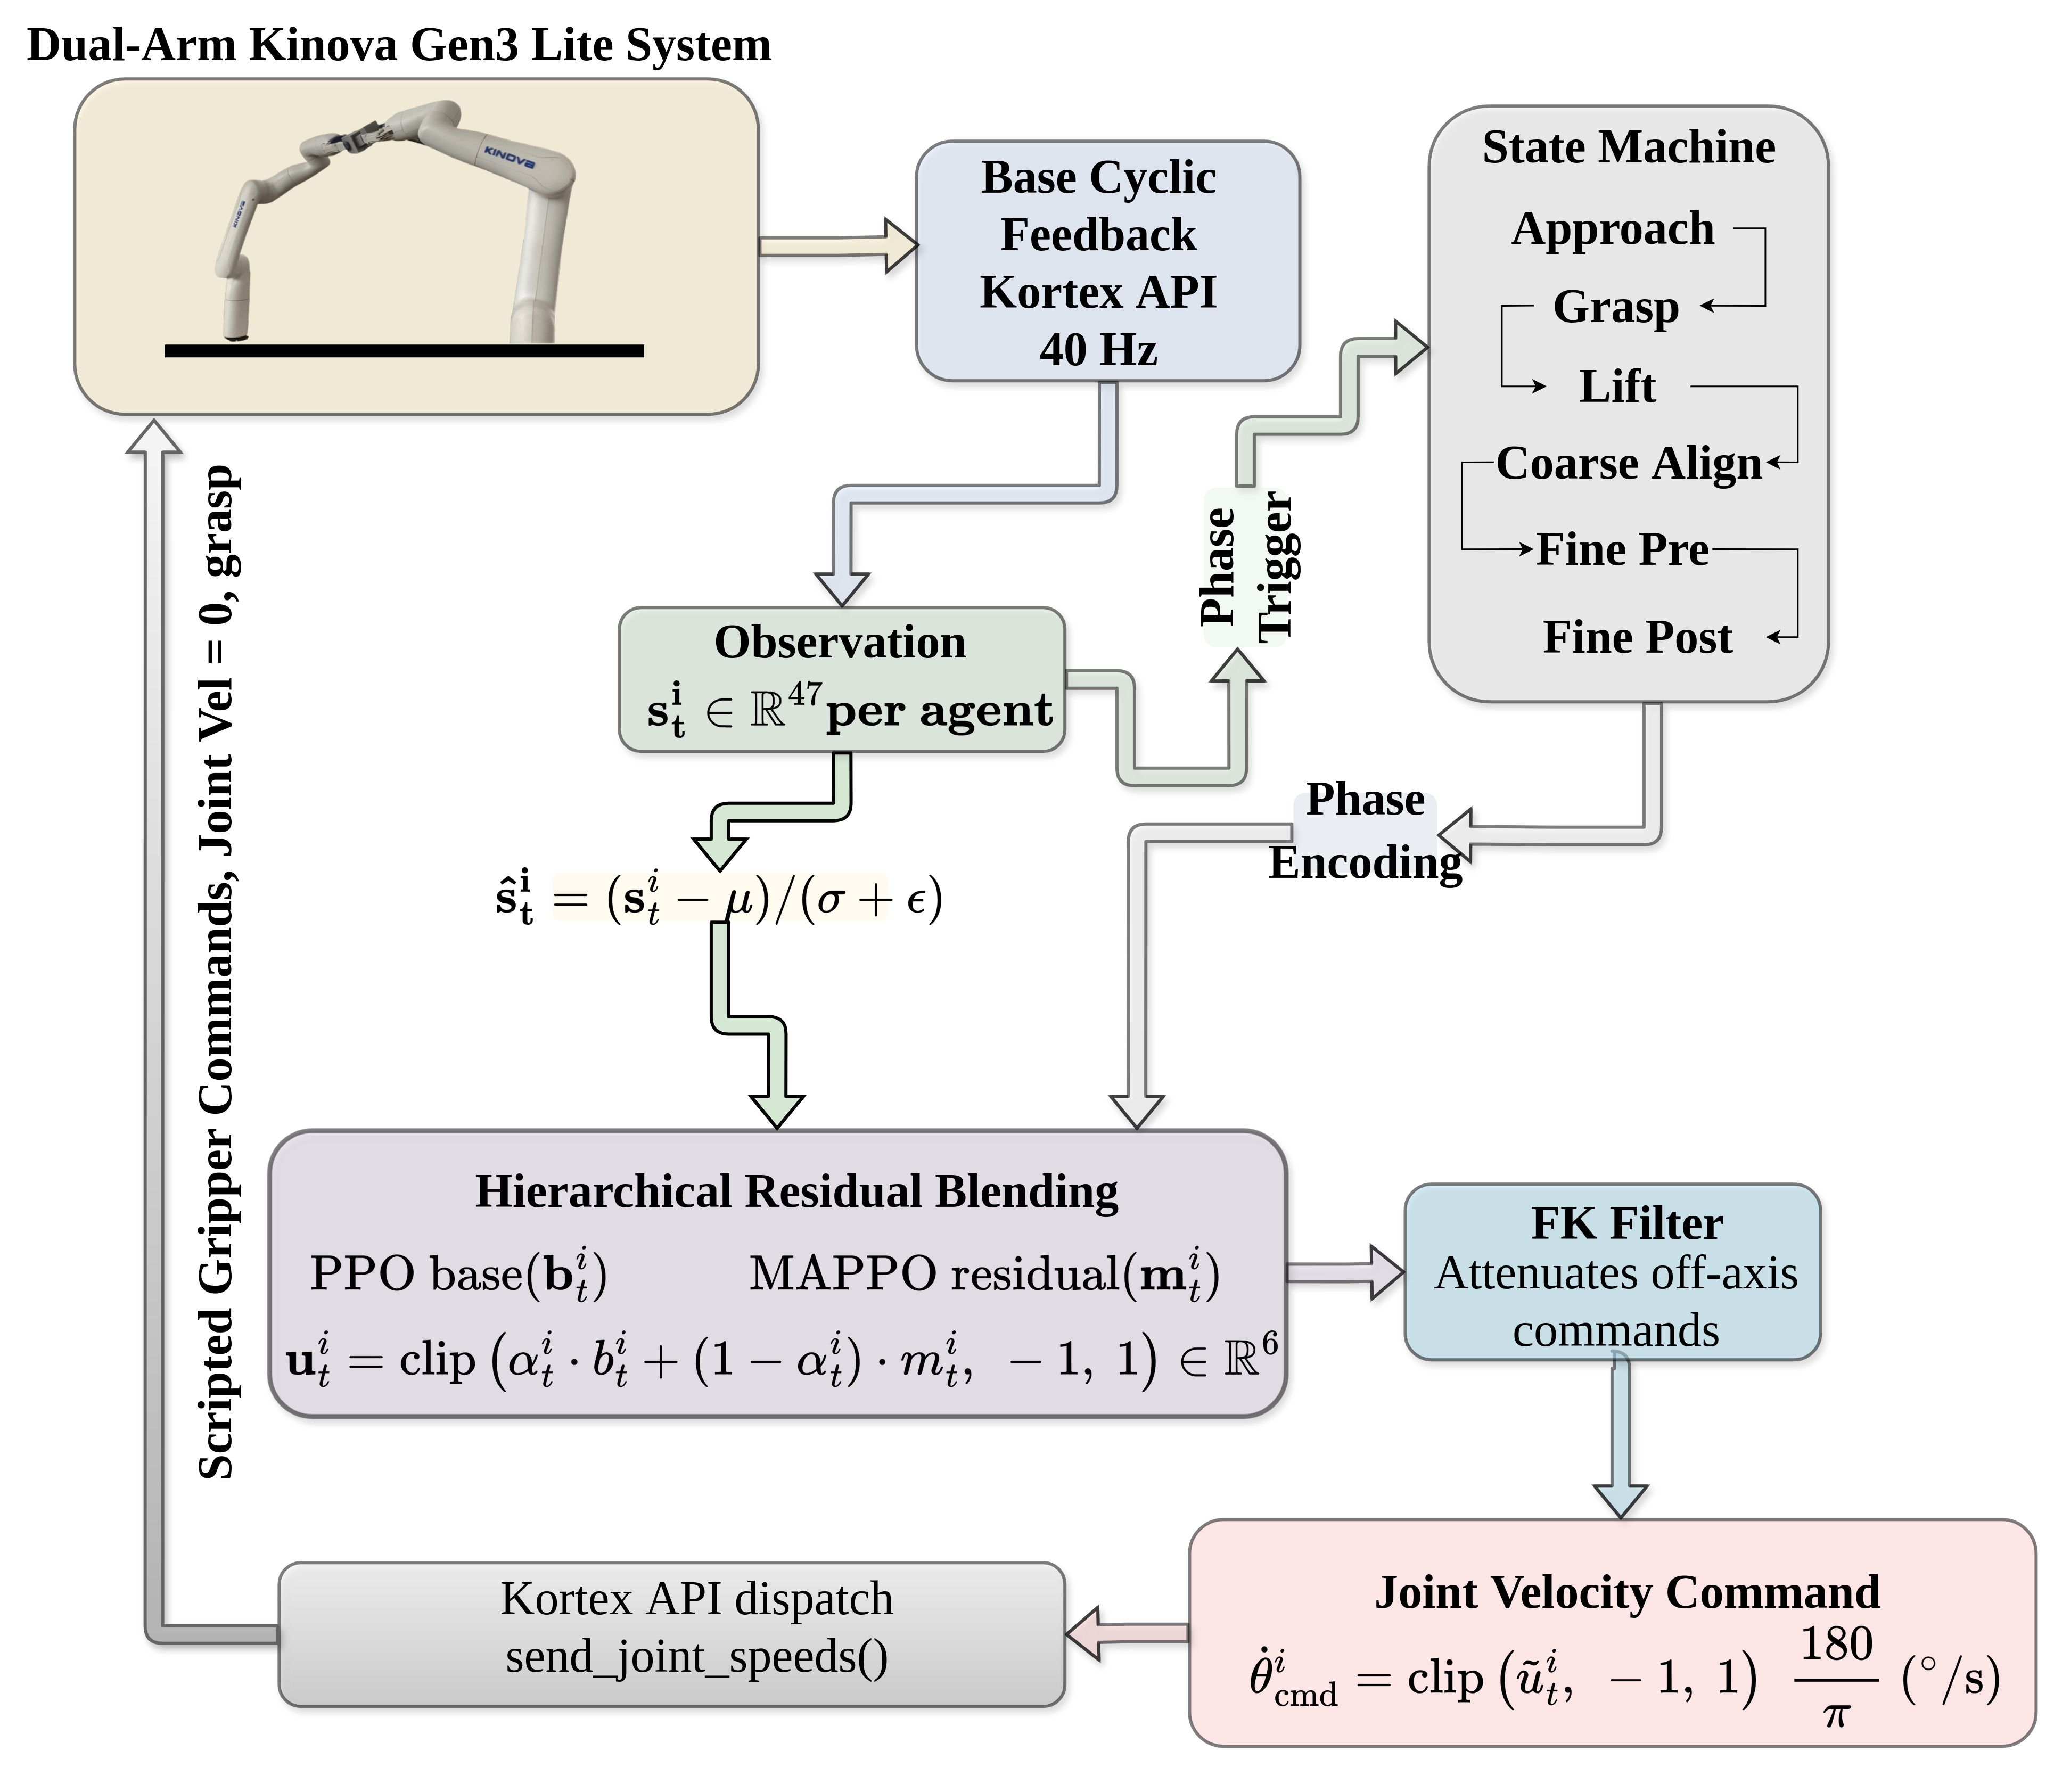
\includegraphics[width=0.75\linewidth]{Images/alpha/Fig_2.jpg}
\caption{Simulation-to-real hardware deployment architecture on the dual Kinova Gen3 Lite
system.}
\label{fig:alpha_sim2real}
\end{figure}

The blended command is scaled and converted to hardware joint velocity commands identically to
Equation~\eqref{eq:dikppo_hwvel} in Part I, and observation normalization statistics, a running mean
and standard deviation over the 47-dimensional local observation, are frozen at the end of training
and applied to every real-hardware observation before inference. The simulation snap mechanism of
Equation~\eqref{eq:alpha_snap} is deliberately not transferred to hardware: without force sensing at
the fingers or active collision avoidance, triggering a proximity-based snap at close range risks
object-to-object or arm-to-arm collision under any residual misalignment. In its place, the state
machine enforces alignment through three predefined spatial-separation waypoints, coarse alignment
at 0.4\,m offset end-effector separation, fine pre-alignment at 0.17\,m, and fine post-alignment at
0.1\,m, progressing to the next waypoint only once both arms simultaneously satisfy the error
thresholds at the current separation. This staged spatial approach removes the need for a dedicated
collision-avoidance module entirely at deployment, and a forward-kinematics consistency check during
fine alignment attenuates velocity commands that deviate significantly from the desired approach
axis as a complementary hardware safety layer, without modifying the policy architecture itself.

%% ============================================================
\section{Results: Baseline, Ablation, and Hardware Validation}\label{sec:alpha_results}
%% ============================================================

Every method in this section was evaluated over 10 independent trials of 4096 parallel environments
each; relative success denotes the conditional alignment rate among environments that already
completed the reach phase.

%% ------------------------------------------------------------
\subsection{Baseline Comparison}\label{subsec:alpha_baseline}
%% ------------------------------------------------------------

\begin{figure}[htbp]
\centering
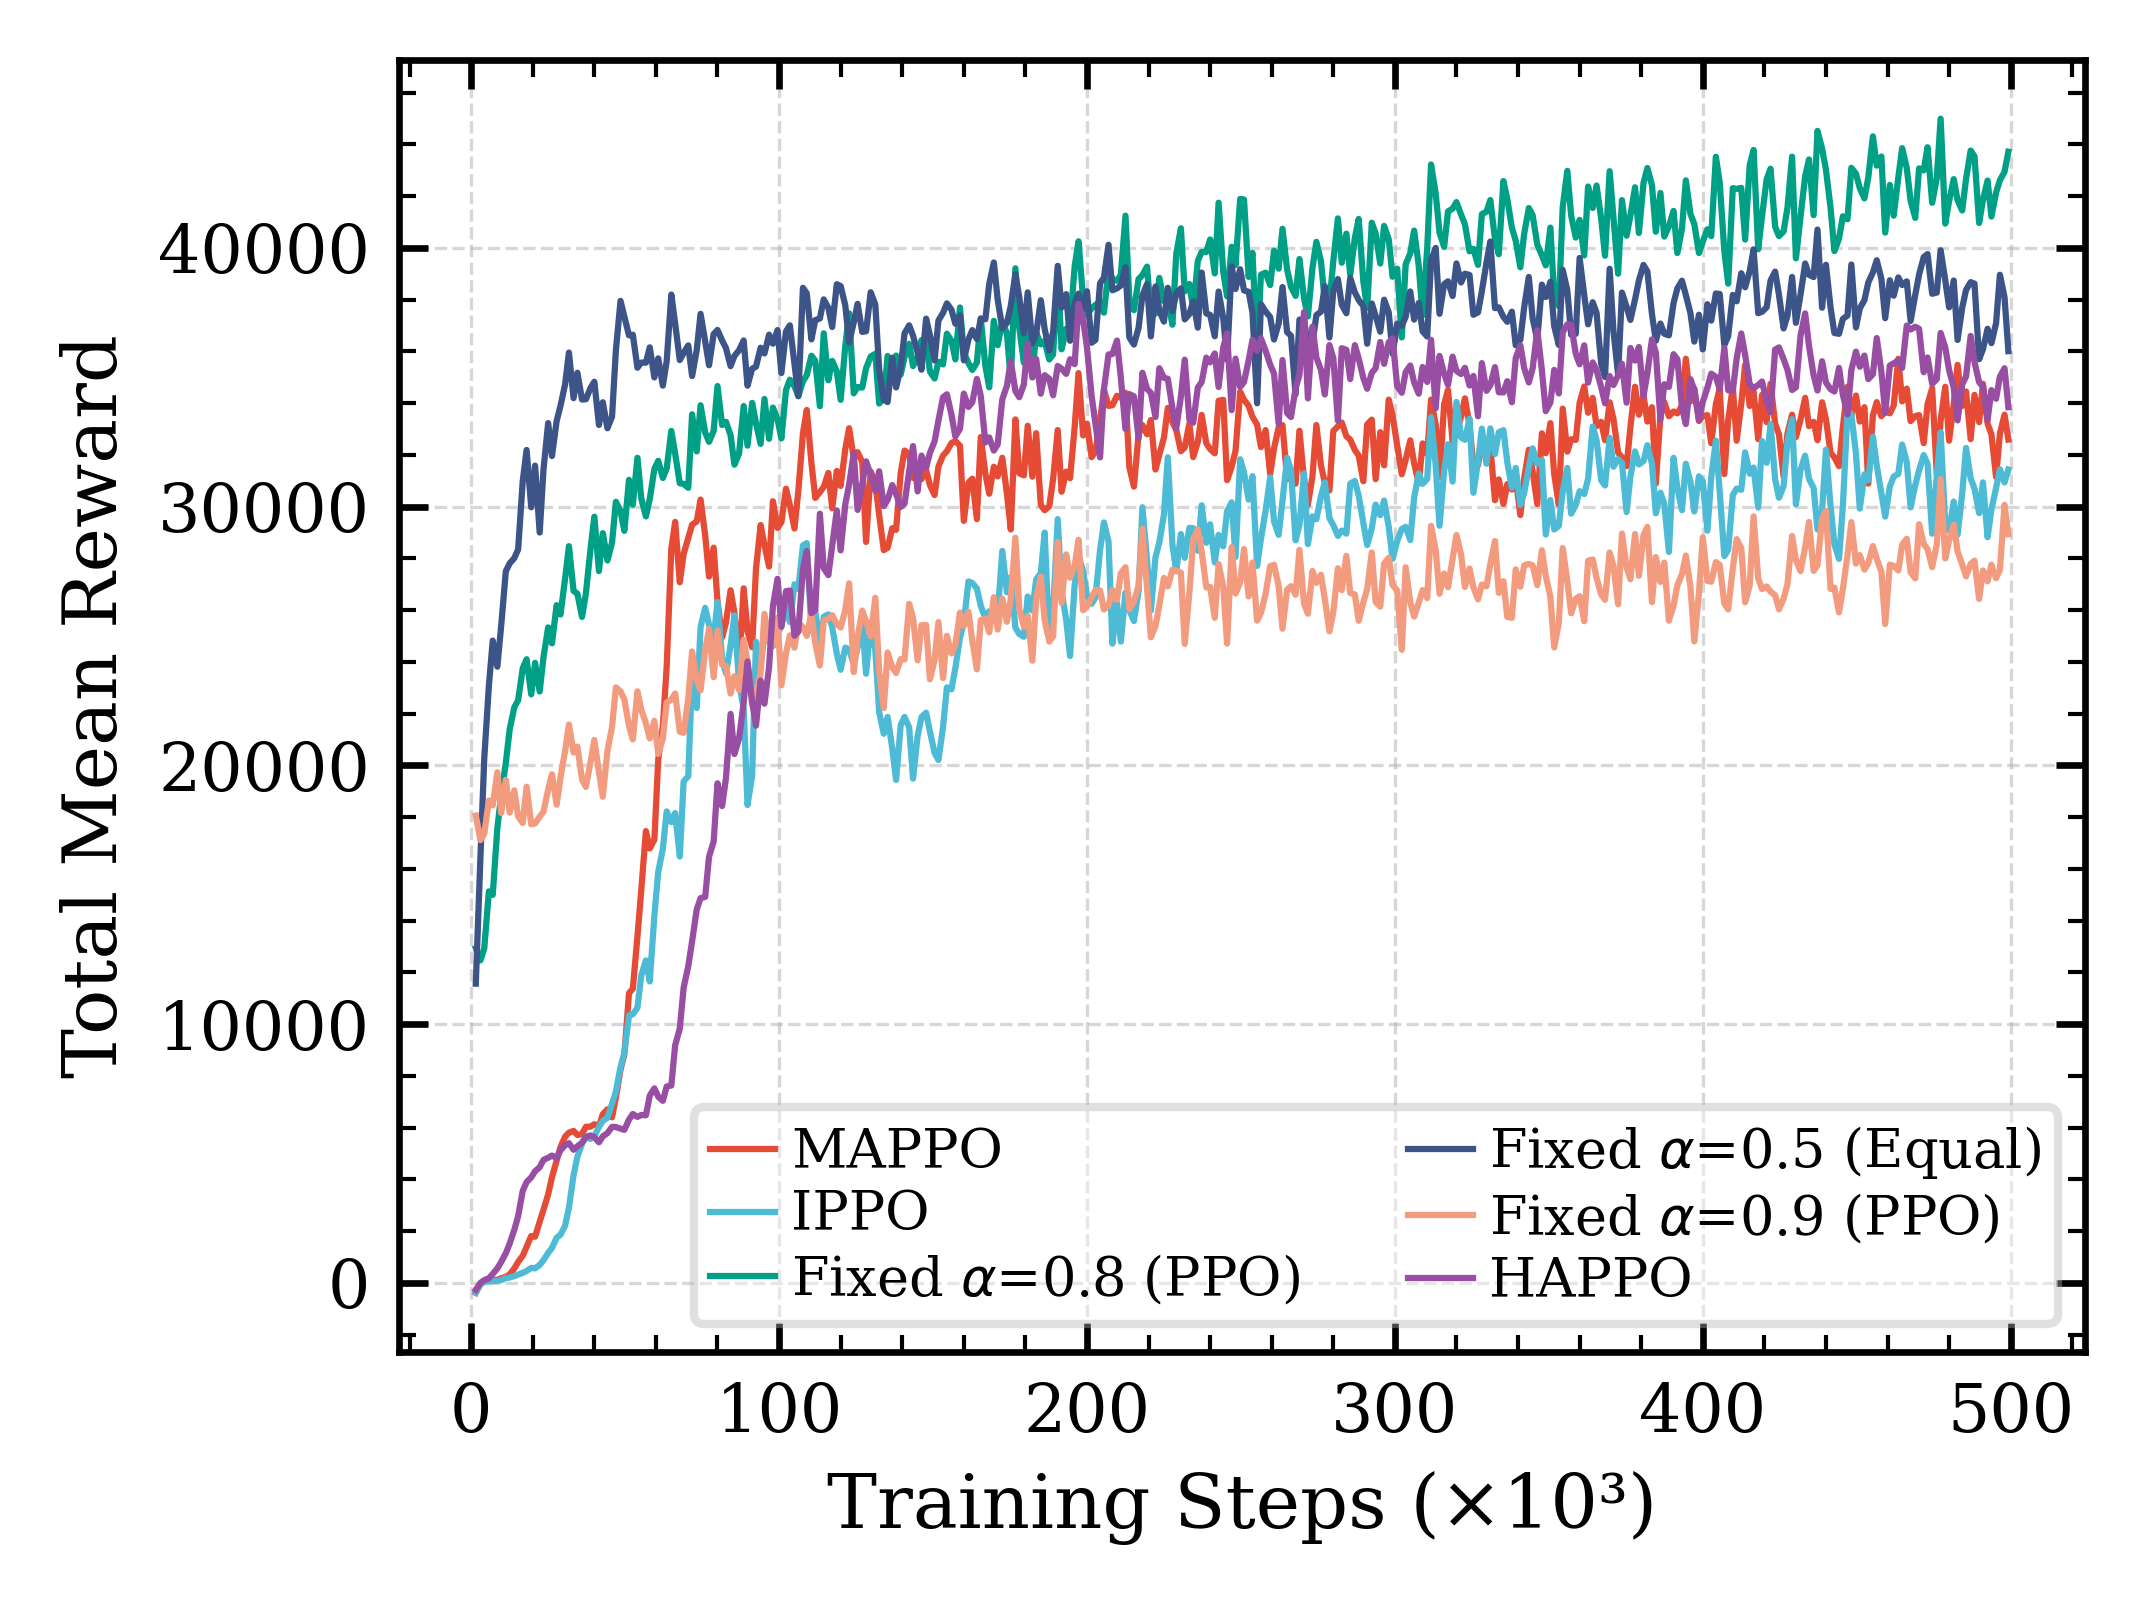
\includegraphics[width=\linewidth]{Images/alpha/Fig_3.png}
% \caption{Baseline comparison: total mean reward evolution of pure MARL algorithms and fixed-ratio
% PPO plus MAPPO blends~\citep{sk2025alpha}.}
\caption{Training reward curves for pure MARL baselines and fixed-blend PPO+MAPPO variants. Curves are Gaussian-smoothed for clarity.}
\label{fig:alpha_baseline}
\end{figure}

\begin{table}[htbp]
\centering
\caption{Evaluation results over 10 trials across 4096 parallel environments (mean $\pm$ std),
comparing ALPHA against pure MARL algorithms and fixed blending
ratios~\citep{sk2025alpha}.}
\label{tab:alpha_baseline}
\resizebox{\textwidth}{!}{%
\begin{tabular}{lccc}
\toprule
\textbf{Method} & \textbf{Reach succ. (\%)} & \textbf{Align succ. (\%)} & \textbf{Rel. succ. (\%)} \\
\midrule
MAPPO~\citep{yu2022surprising}                 & 71.6 $\pm$ 0.5 & 8.3 $\pm$ 0.3 & 11.6 $\pm$ 0.5 \\
HAPPO~\citep{kuba2021trust}                    & \textbf{73.6 $\pm$ 0.7} & \textbf{32.3 $\pm$ 0.8} & 43.9 $\pm$ 1.2 \\
IPPO~\citep{dewitt2020independent}             & 62.0 $\pm$ 0.5 & 25.0 $\pm$ 0.3 & 40.3 $\pm$ 0.6 \\
HATRPO~\citep{kuba2021trust}                   & 6.6 $\pm$ 0.3  & 3.4 $\pm$ 0.1  & 51.5 $\pm$ 2.8 \\
PPO-MAPPO (0.5-0.5, fixed)                     & 41.1 $\pm$ 0.8 & 18.4 $\pm$ 0.5 & 44.8 $\pm$ 1.1 \\
PPO-MAPPO (0.8-0.2, fixed)                     & 47.7 $\pm$ 0.8 & 17.6 $\pm$ 0.8 & 36.9 $\pm$ 1.3 \\
PPO-MAPPO (0.9-0.1, fixed)                     & 1.76 $\pm$ 0.2 & 0.02 $\pm$ 0.01 & 1.1 $\pm$ 0.6 \\
\bottomrule
\end{tabular}%
}
\end{table}

Table~\ref{tab:alpha_baseline} and Figure~\ref{fig:alpha_baseline} expose the fundamental sample
complexity cost of learning reachability and coordination together. Pure MAPPO reaches the highest
reach success (71.6\%) but collapses to 8.3\% alignment, since learning low-level reachability and
high-level alignment simultaneously under a single joint reward degrades sample efficiency sharply.
IPPO, despite being blind to the partner agent's state, achieves higher absolute alignment (25.0\%)
than MAPPO, indicating that decentralized critics encourage more conservative per-arm behaviour that
reduces interference during fine alignment, at the direct cost of coordination quality. HAPPO
reaches the highest reach success among MARL baselines (73.6\%) but its sequential per-agent update,
the mechanism providing its monotonic-improvement guarantee, computes one agent's advantage against
an already-shifted joint policy for the other, directly disrupting the simultaneous convergence
bilateral alignment demands. HATRPO collapses almost entirely (6.6\% reach), its exact
KL-constrained update proving incompatible with 12-DOF continuous joint velocity exploration.
Fixed-ratio blending reveals a further, counterintuitive decoupling: despite the highest cumulative
training reward of any configuration, fixed $\alpha = 0.8$ and $\alpha = 0.5$ yield reach success of
only 47.7\% and 41.1\%, since a rigidly dominant prior actively suppresses the coordination policy's
capacity to enforce alignment, while $\alpha = 0.9$ collapses reach success to 1.76\% despite
retaining among the highest reward curves, demonstrating directly that cumulative reward is an
unreliable proxy for cooperative task success whenever the base policy dominates the action space.

%% ------------------------------------------------------------
\subsection{Ablation Study}\label{subsec:alpha_ablation}
%% ------------------------------------------------------------

\begin{figure}[htbp]
\centering
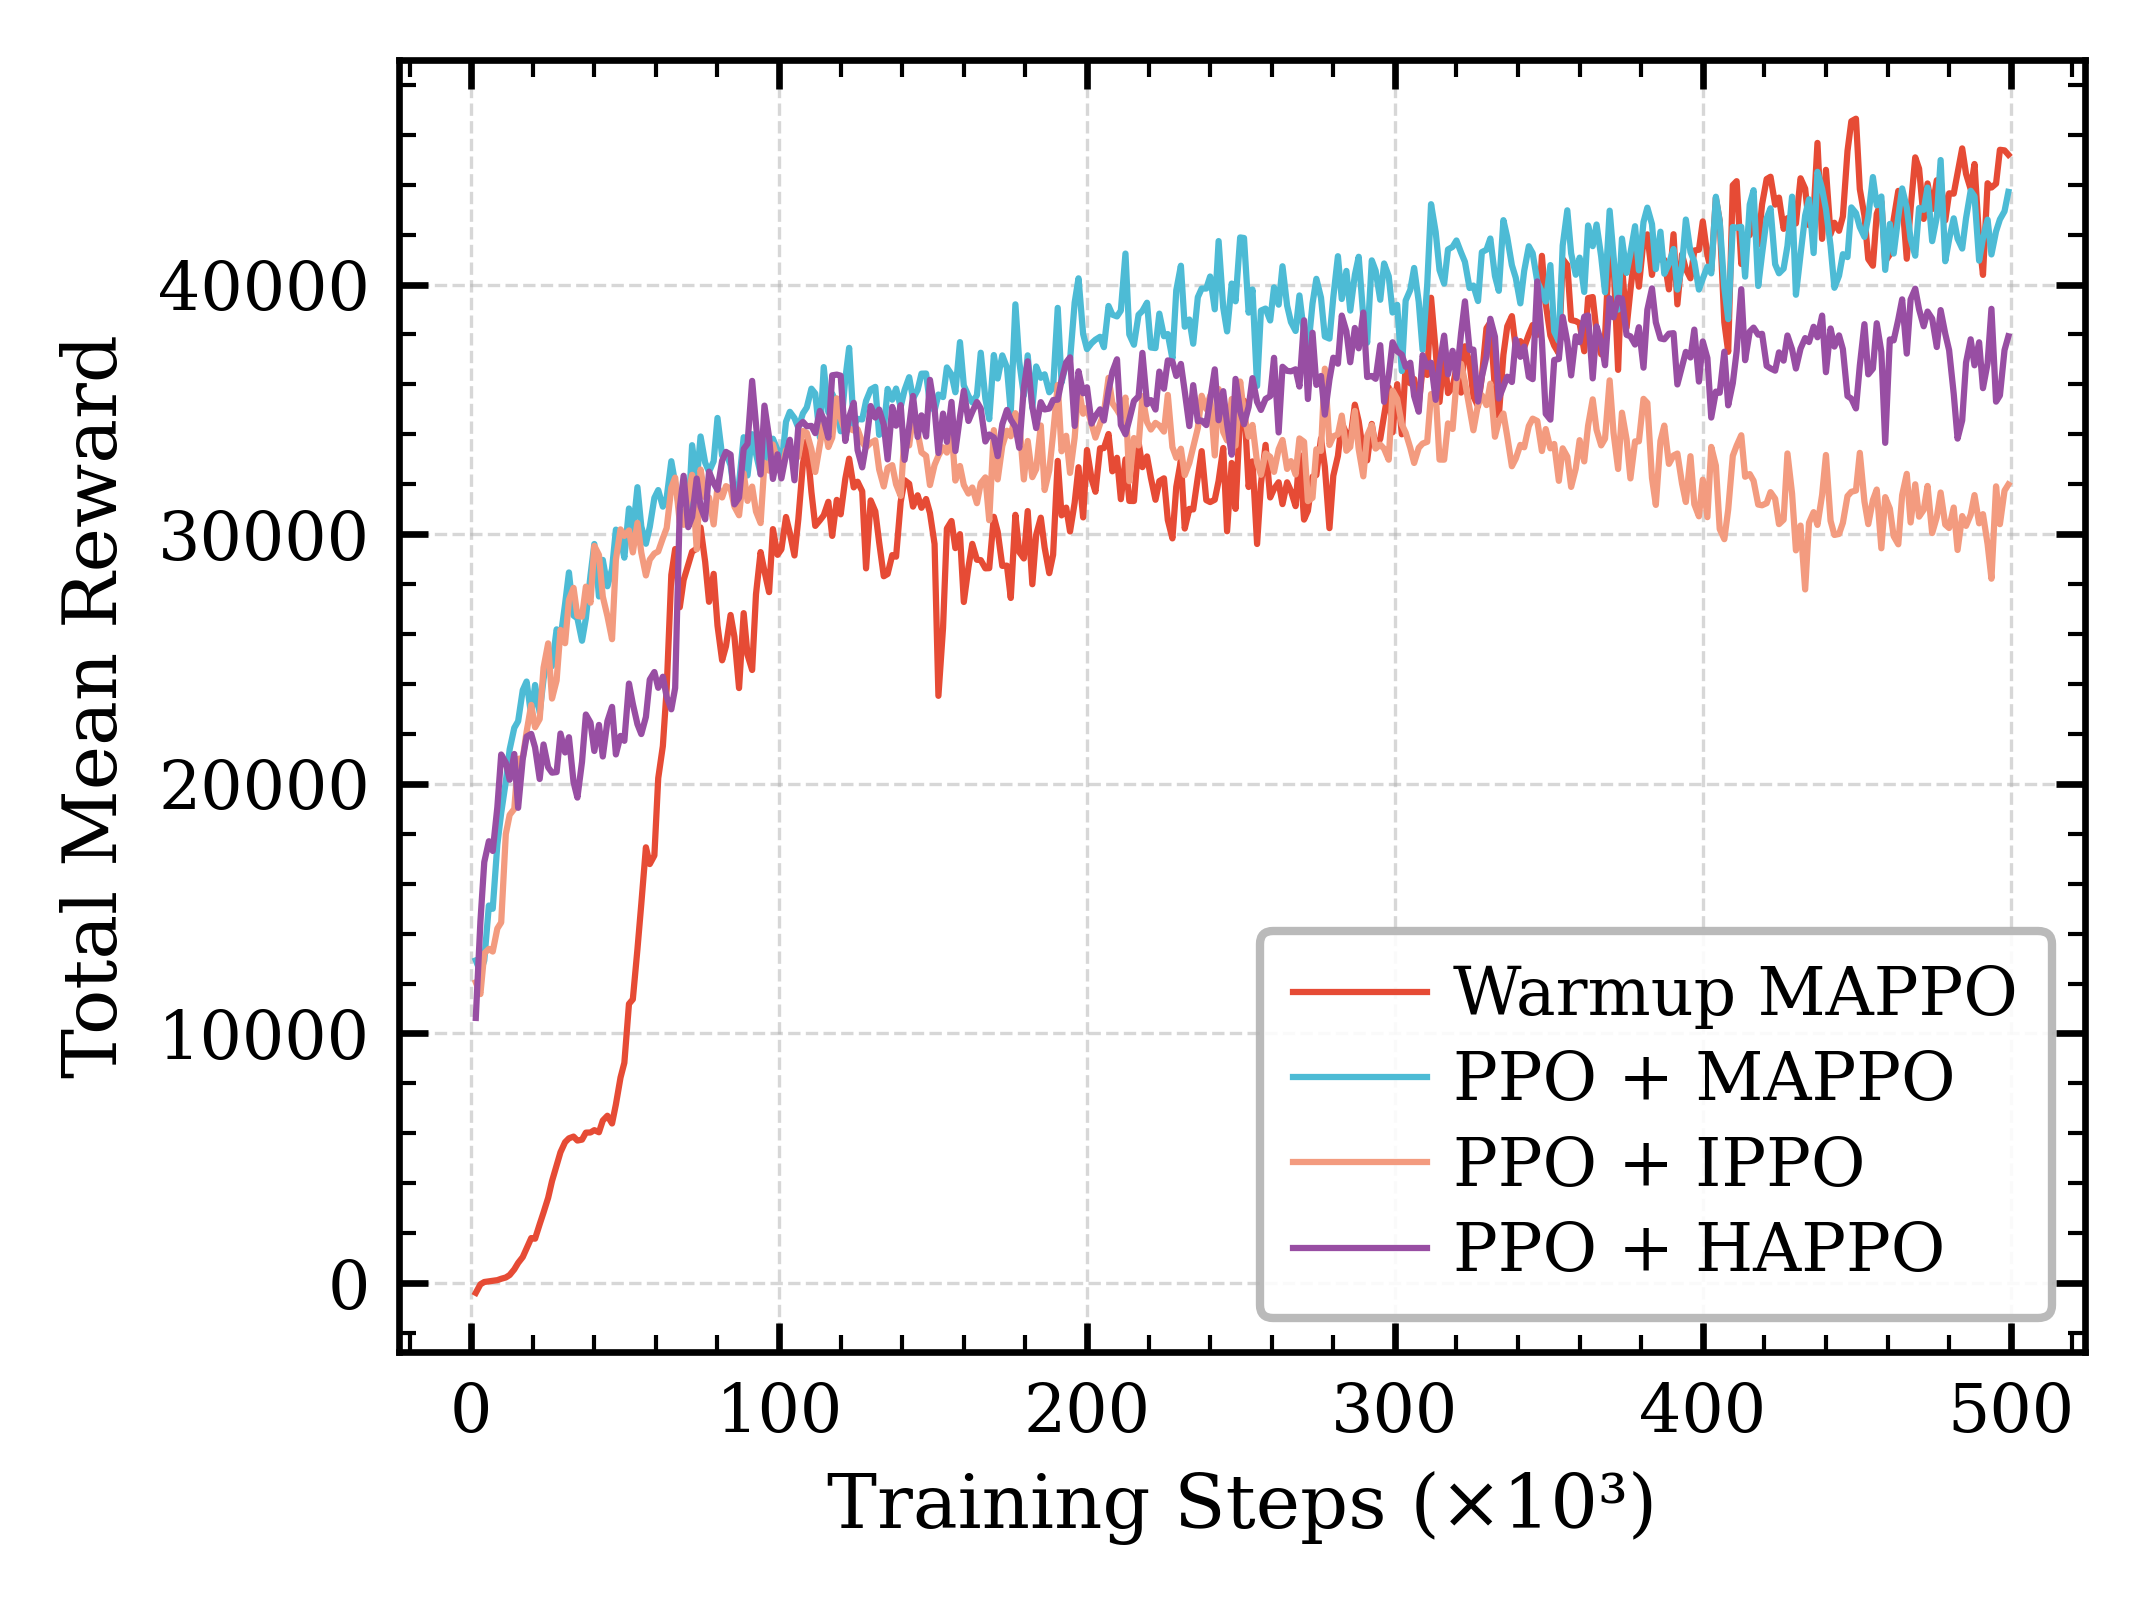
\includegraphics[width=\linewidth]{Images/alpha/Fig_4.png}
\caption{Ablation study: total mean reward evolution of ALPHA (adaptive PPO plus MAPPO from
timestep zero) against a warm-up curriculum (150k-step scale freeze) and adaptive blending with alternative MARL algorithms.}
\label{fig:alpha_ablation}
\end{figure}

\begin{table}[h]
\caption{Ablation study results over 10 trials across 4,096 parallel environments(Mean $\pm$ Std)}
\centering
\resizebox{\columnwidth}{!}{
\begin{tabular}{lccc}
\midrule 
\textbf{Method} & \textbf{Reach Succ(\%)} & \textbf{Align Succ(\%)} & \textbf{Rel.Succ(\%)} \\
\midrule \midrule
Warmup MAPPO & 88.50$\pm$0.3& 85.80$\pm$0.2 & 96.94$\pm$0.3\\
\textbf{PPO + MAPPO (ours)} & \textbf{96.50$\pm$0.3} & \textbf{95.0$\pm$0.4} & \textbf{98.45$\pm$0.4}\\
PPO + IPPO  & 67.50$\pm$0.7& 62.50$\pm$0.9 & 92.60$\pm$1.2\\
PPO + HAPPO & 92$\pm$0.2 & 87$\pm$0.4 & 94.60$\pm$0.5\\
\midrule
\end{tabular}}
\vspace{2pt}
    \footnotesize{\textit{Note*:}} \textit{All variants were trained under a single seed (42); the reported deviations therefore characterize evaluation variance at fixed initialization. Seed-level variance for the proposed method is reported in Table~\ref{tab:seed_robustness}.}
\label{tab:alpha_ablation}
\end{table}

\begin{table}[h]
\caption{Seed robustness of PPO+MAPPO (Adaptive) and of the $\alpha$-detached control. Each seed evaluated over 10 independent trials across 4,096 parallel environments (Mean $\pm$ Std across trials). Each block's final row reports Mean $\pm$ Std across the three training seeds.}
\centering
\resizebox{\columnwidth}{!}{
\begin{tabular}{lccc}
\midrule
\textbf{Training Seed} & \textbf{Reach Succ(\%)} & \textbf{Align Succ(\%)} & \textbf{Rel.Succ(\%)} \\
\midrule \midrule
42  & 96.54$\pm$0.37 & 95.07$\pm$0.49 & 98.47$\pm$0.21 \\
100 & 95.81$\pm$0.29 & 93.48$\pm$0.42 & 97.57$\pm$0.27 \\
200 & 95.40$\pm$0.49 & 93.03$\pm$0.42 & 97.52$\pm$0.18 \\
\midrule
\textbf{Across seeds} & \textbf{95.92$\pm$0.58} & \textbf{93.86$\pm$1.07} & \textbf{97.86$\pm$0.53} \\
\midrule \midrule
\multicolumn{4}{l}{\textit{PPO+MAPPO ($\alpha$-detached)}} \\
\midrule
42  & 81.80$\pm$0.62 & 49.86$\pm$0.56 & 60.96$\pm$0.92 \\
100 & 81.74$\pm$0.50 & 59.78$\pm$0.55 & 73.13$\pm$0.86 \\
200 & 81.47$\pm$0.74 & 69.24$\pm$0.87 & 84.99$\pm$0.54 \\
\midrule
\textbf{Across seeds} & \textbf{81.67$\pm$0.18} & \textbf{59.62$\pm$9.69} & \textbf{73.03$\pm$12.02} \\
\midrule
\end{tabular}}
\label{tab:seed_robustness}
\end{table}

% \begin{table}[htbp]
% \centering
% \caption{Ablation study over 10 trials across 4096 parallel environments (mean $\pm$
% std)~\citep{sk2025alpha}.}
% \label{tab:alpha_ablation}
% \resizebox{\textwidth}{!}{%
% \begin{tabular}{lccc}
% \toprule
% \textbf{Method} & \textbf{Reach succ. (\%)} & \textbf{Align succ. (\%)} & \textbf{Rel. succ. (\%)} \\
% \midrule
% Warm-up MAPPO ($\alpha$ frozen at 0 for 150k steps) & 88.50 $\pm$ 0.3 & 85.80 $\pm$ 0.2 & 96.94 $\pm$ 0.3 \\
% \textbf{ALPHA (PPO-MAPPO, adaptive from $t=0$)}      & \textbf{96.50 $\pm$ 0.3} & \textbf{95.0 $\pm$ 0.4} & \textbf{98.45 $\pm$ 0.4} \\
% PPO-IPPO (adaptive)                                    & 67.50 $\pm$ 0.7 & 62.50 $\pm$ 0.9 & 92.60 $\pm$ 1.2 \\
% PPO-HAPPO (adaptive)                                     & 92 $\pm$ 0.2 & 87 $\pm$ 0.4 & 94.60 $\pm$ 0.5 \\
% PPO-HATRPO (adaptive)                                      & 63.4 $\pm$ 0.7 & 42.4 $\pm$ 0.9 & 66.90 $\pm$ 1.6 \\
% \bottomrule
% \end{tabular}%
% }
% \end{table}

Table~\ref{tab:alpha_ablation} and Figure~\ref{fig:alpha_ablation} isolate the individual
contributions of adaptive blending, centralized training, and the warm-up curriculum. ALPHA achieves
the highest performance across every metric (96.5\% reach, 95.0\% alignment, 98.45\% relative
success), confirming that adaptive $\alpha_t^i$ combined with CTDE is the strongest configuration.
Replacing MAPPO with IPPO under the identical adaptive blending mechanism drops alignment to 62.5\%,
directly isolating the centralized critic's contribution: without global state access during
training, the decentralized coordination policy cannot learn the precise bilateral coordination
alignment convergence requires. PPO-HAPPO reaches 92\% and 87\%, confirming that adaptive blending
partially compensates for the absence of a fully centralized critic, though the residual 8\%
alignment gap to ALPHA persists since HAPPO's factored advantage estimates cannot fully substitute
for genuinely global bilateral state. The warm-up variant, which freezes $\alpha_t^i$ at zero for the
first 150k timesteps before enabling adaptive blending, reaches 85.8\% alignment, underperforming
ALPHA by $\approx 9$ points despite eventually reaching the same adaptive mechanism, its reward curve
in Figure~\ref{fig:alpha_ablation} shows a pronounced dip and delayed recovery around the transition
point, indicating that introducing blending abruptly after a pure-MAPPO warm-up disrupts an already
established policy in a way that co-adapting from timestep zero avoids.

\begin{figure}[htbp]
\centering
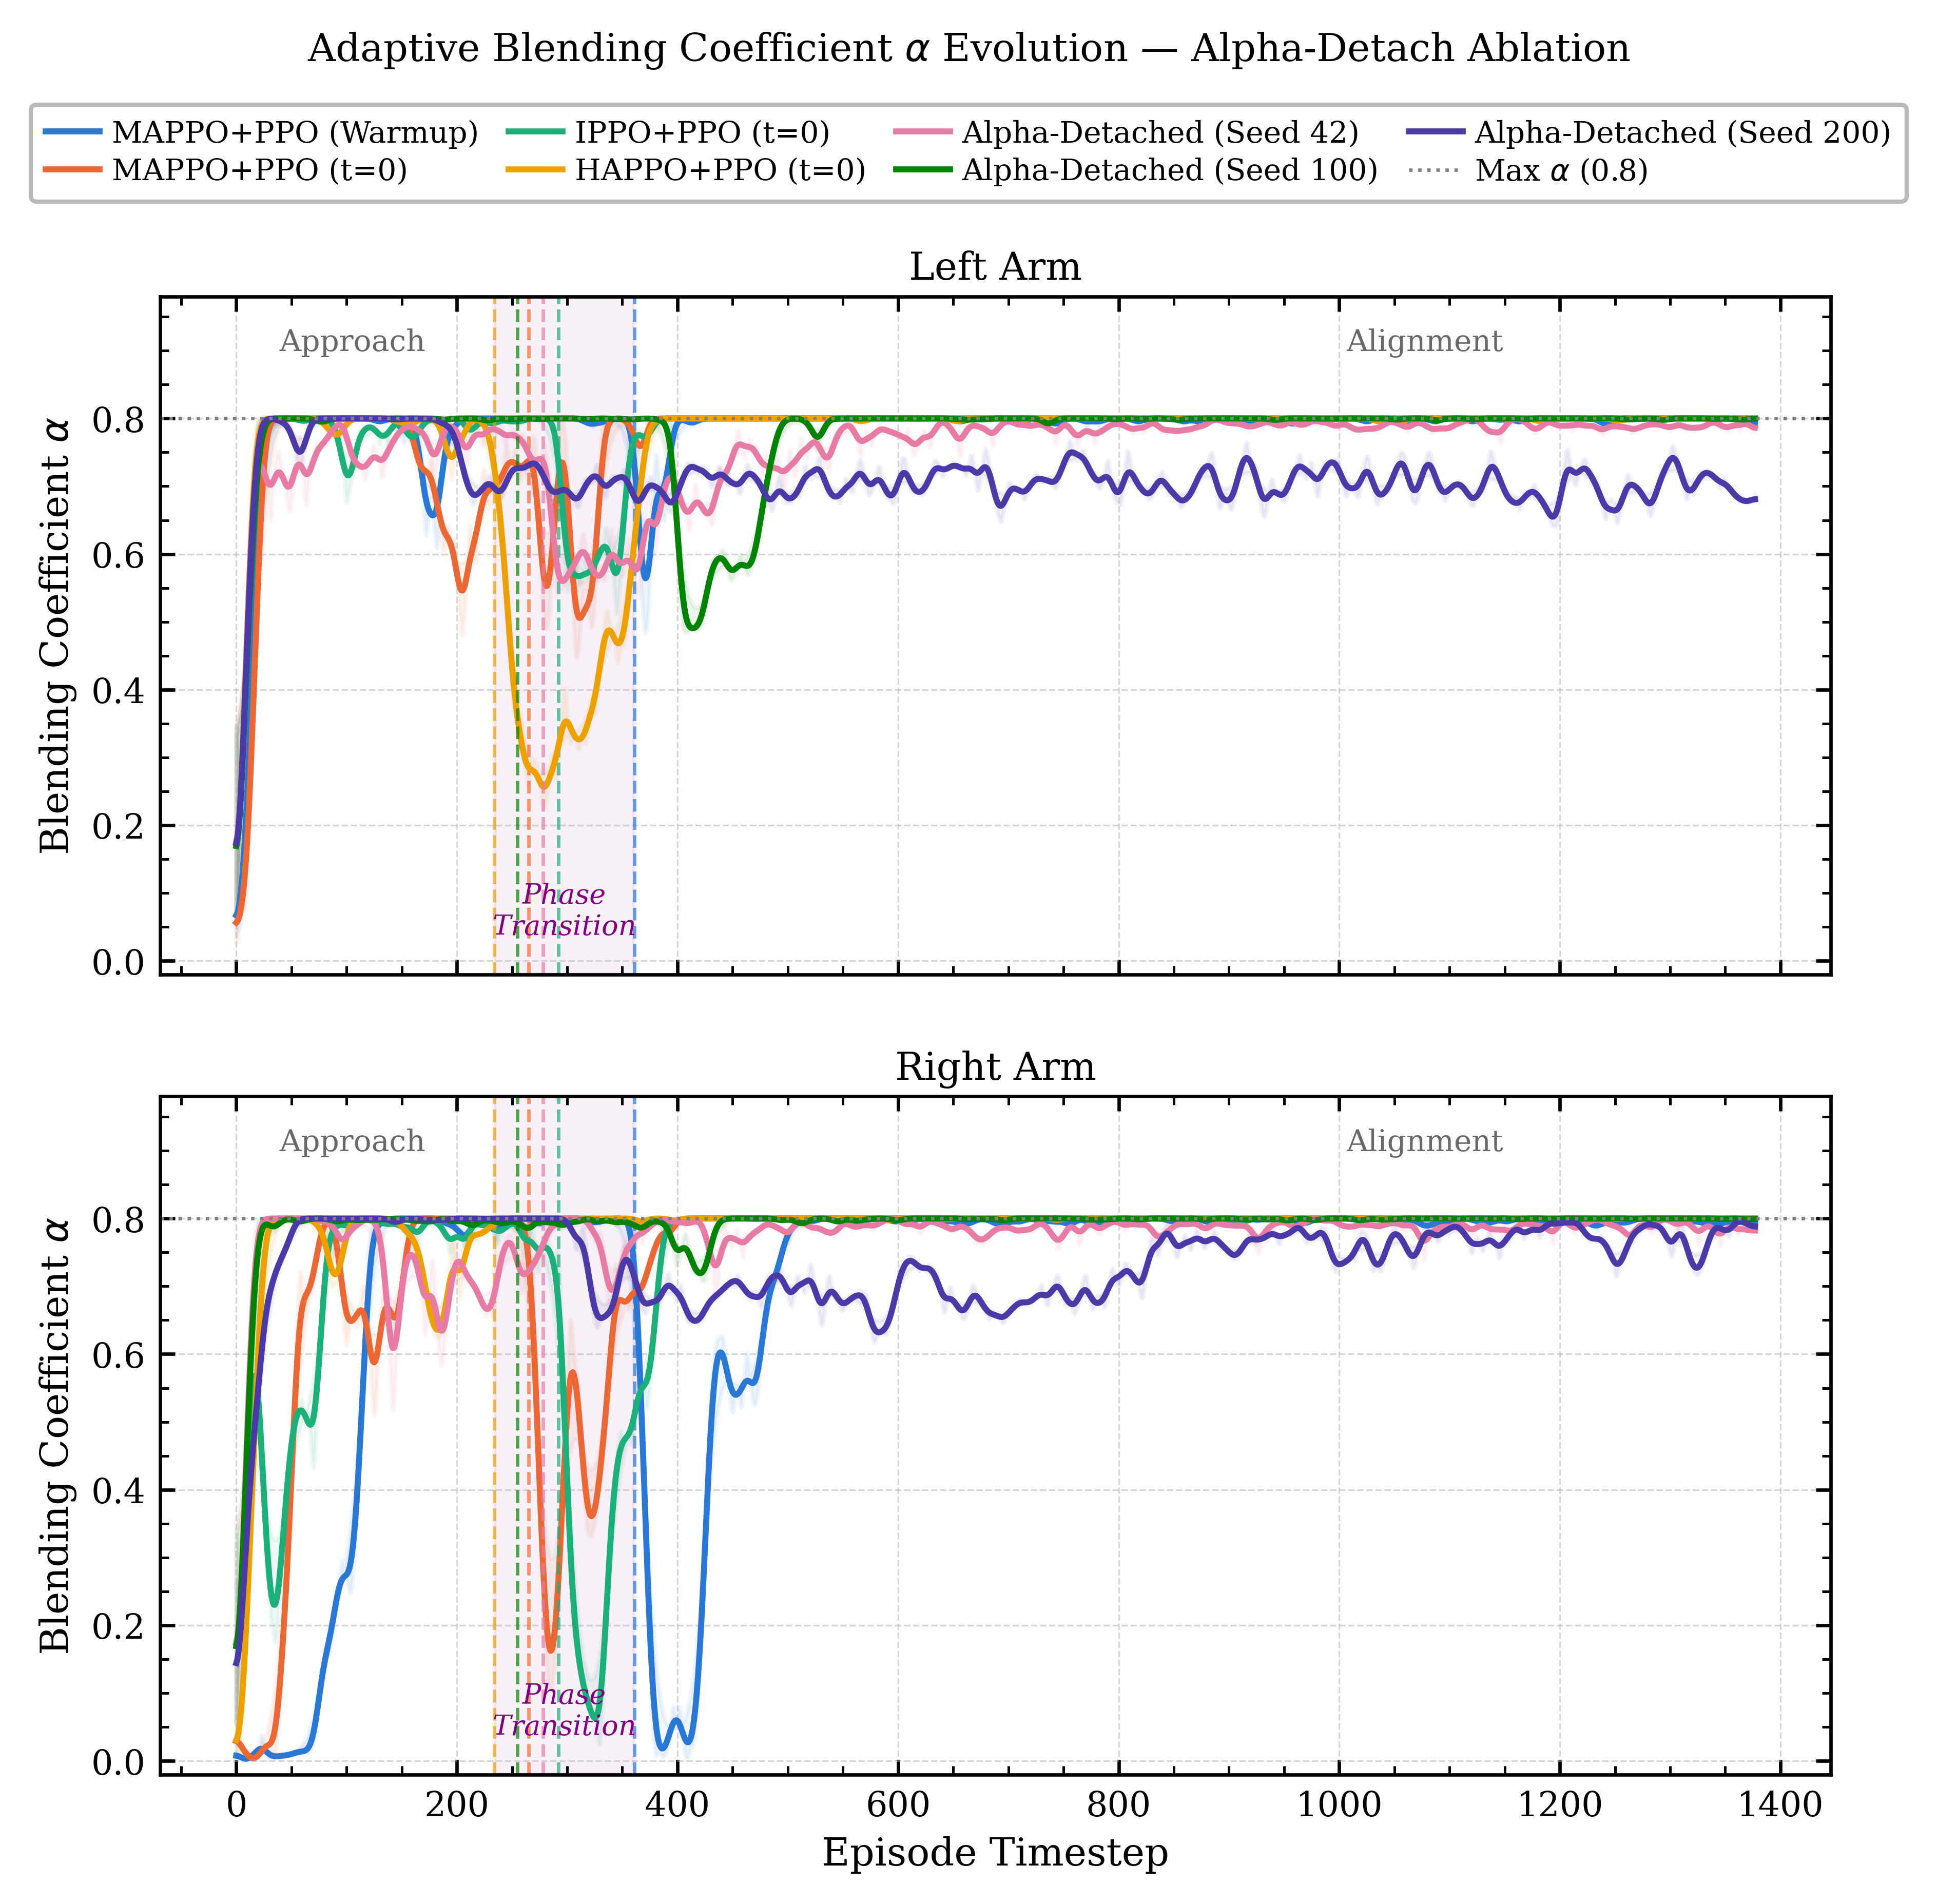
\includegraphics[width=\linewidth]{Images/alpha/Fig_5.png}
% \caption{Comparison of methods' adaptive scale $\alpha_t^i$ evolution over a single
% episode~\citep{sk2025alpha}.}
\caption{Adaptive blending coefficient $\alpha^i_t$ evolution over a single episode for both arms across all trained variants, alongside the $\alpha$-detached control under each of its three training seeds.}
\label{fig:alpha_evolution}
\end{figure}

Figure~\ref{fig:alpha_evolution} shows $\alpha_t^i$ evolving across a single episode for both arms.
During approach, every method rapidly saturates $\alpha_t^i$ toward 0.8, confirming the policy
learns to defer maximally to the frozen prior for single-arm reaching; at the phase transition,
every method shows a pronounced reduction in $\alpha_t^i$, actively suppressing prior reliance
exactly when cooperative alignment demands coordinated deviation from independent reaching, which is
the direct empirical justification for adaptive rather than fixed blending, since any fixed
$\alpha_t^i$ would retain inappropriate prior dominance precisely at this transition. ALPHA shows
the shallowest and shortest dip on both arms of any method, recovering fastest due to the centralized
critic's global coordination signal, while PPO-IPPO's dip is deeper and oscillatory, consistent with
its decentralized critic being unable to resolve coupled bilateral alignment without global state
access.

%% ------------------------------------------------------------
\subsection{Hardware Validation}\label{subsec:alpha_hardware}
%% ------------------------------------------------------------

\begin{figure}[htbp]
\centering
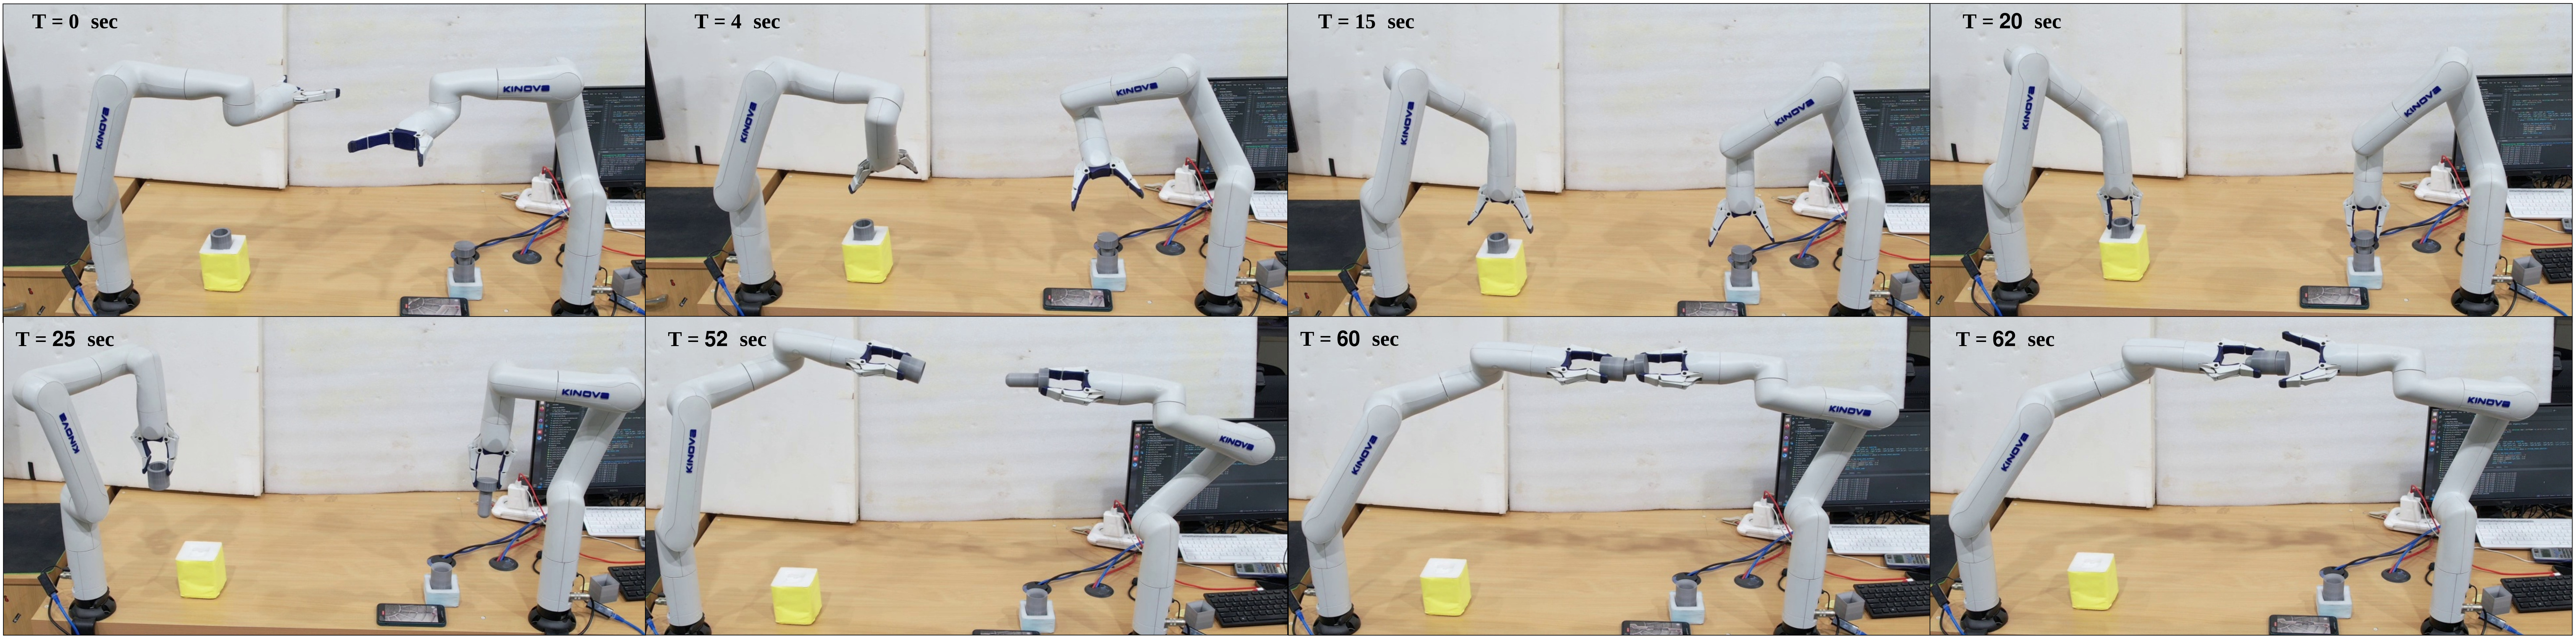
\includegraphics[width=\linewidth]{Images/alpha/hardware_exp1_cylinder.jpg}
\caption{Experiment 1: sequential execution of the dual-arm pick-and-pre-assembly alignment task for
a cylindrical peg and hole on physical Kinova Gen3 Lite hardware.}
\label{fig:alpha_exp1}
\end{figure}

\begin{figure}[htbp]
\centering
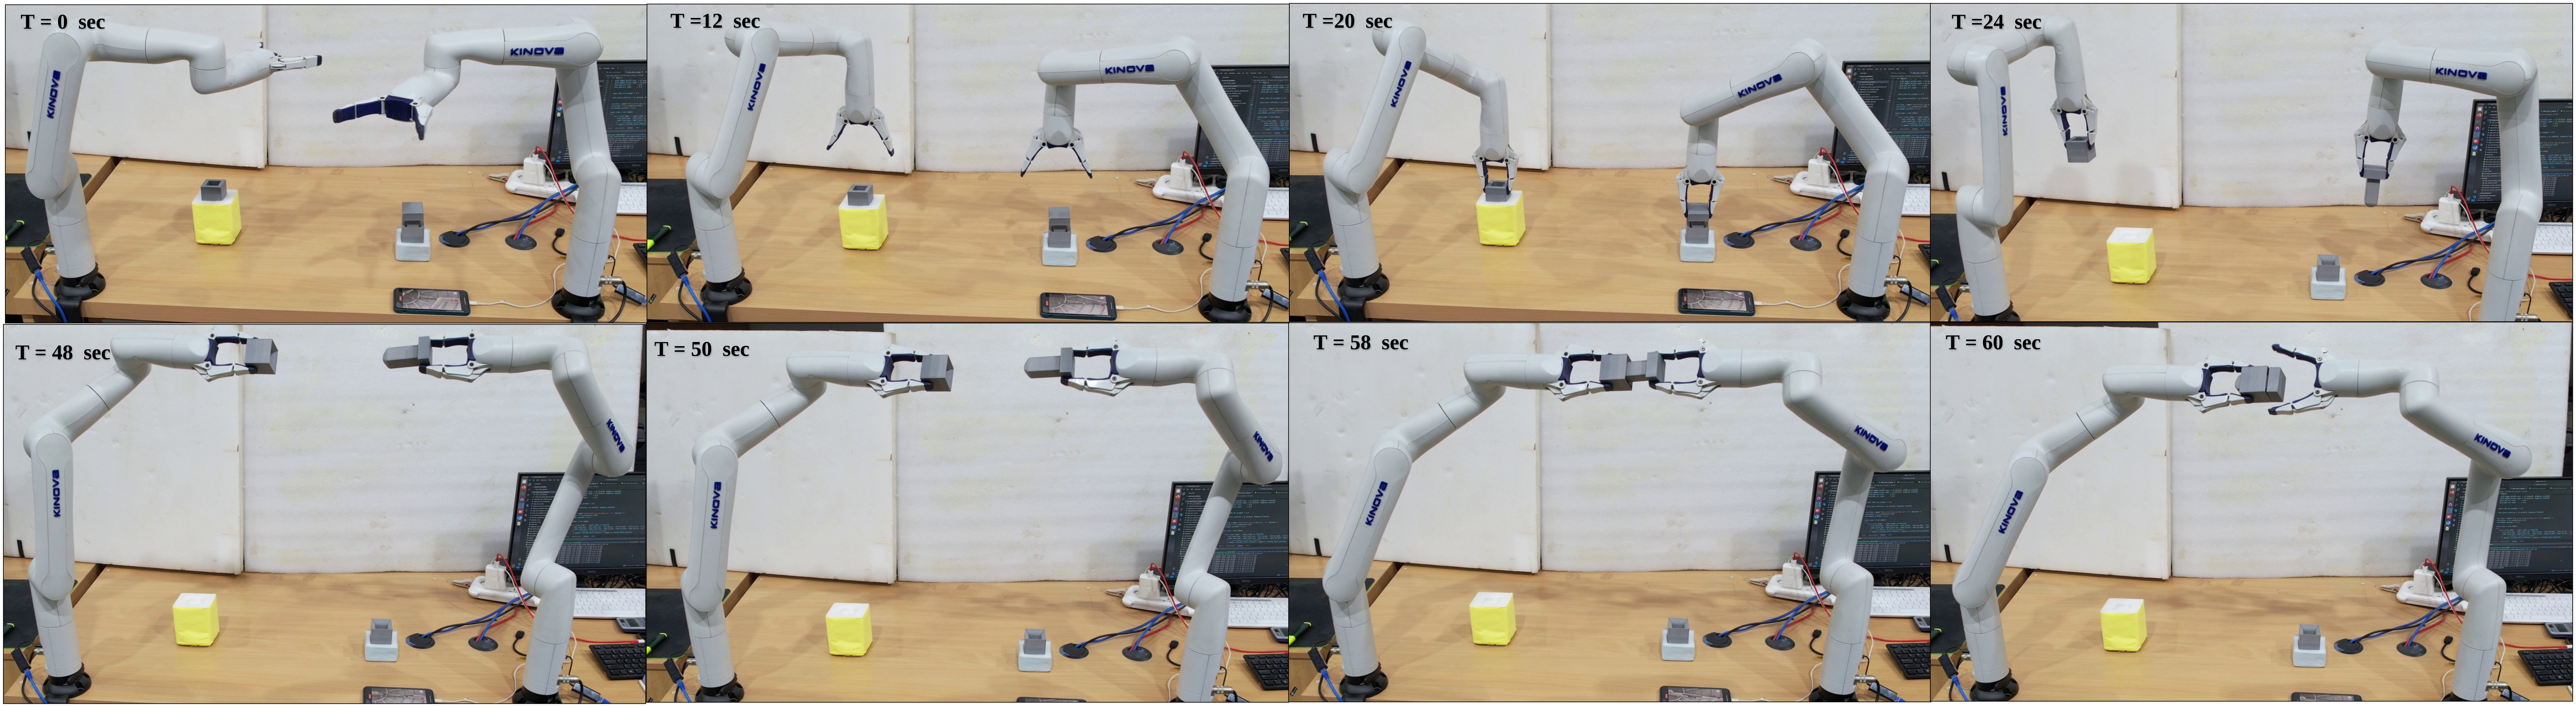
\includegraphics[width=\linewidth]{Images/alpha/hardware_exp2_square.jpg}
\caption{Experiment 2: sequential execution of the dual-arm pick-and-pre-assembly alignment task for a square peg and hole on physical Kinova Gen3 Lite hardware.}
\label{fig:alpha_exp2}
\end{figure}

\begin{figure}[htbp]
\centering
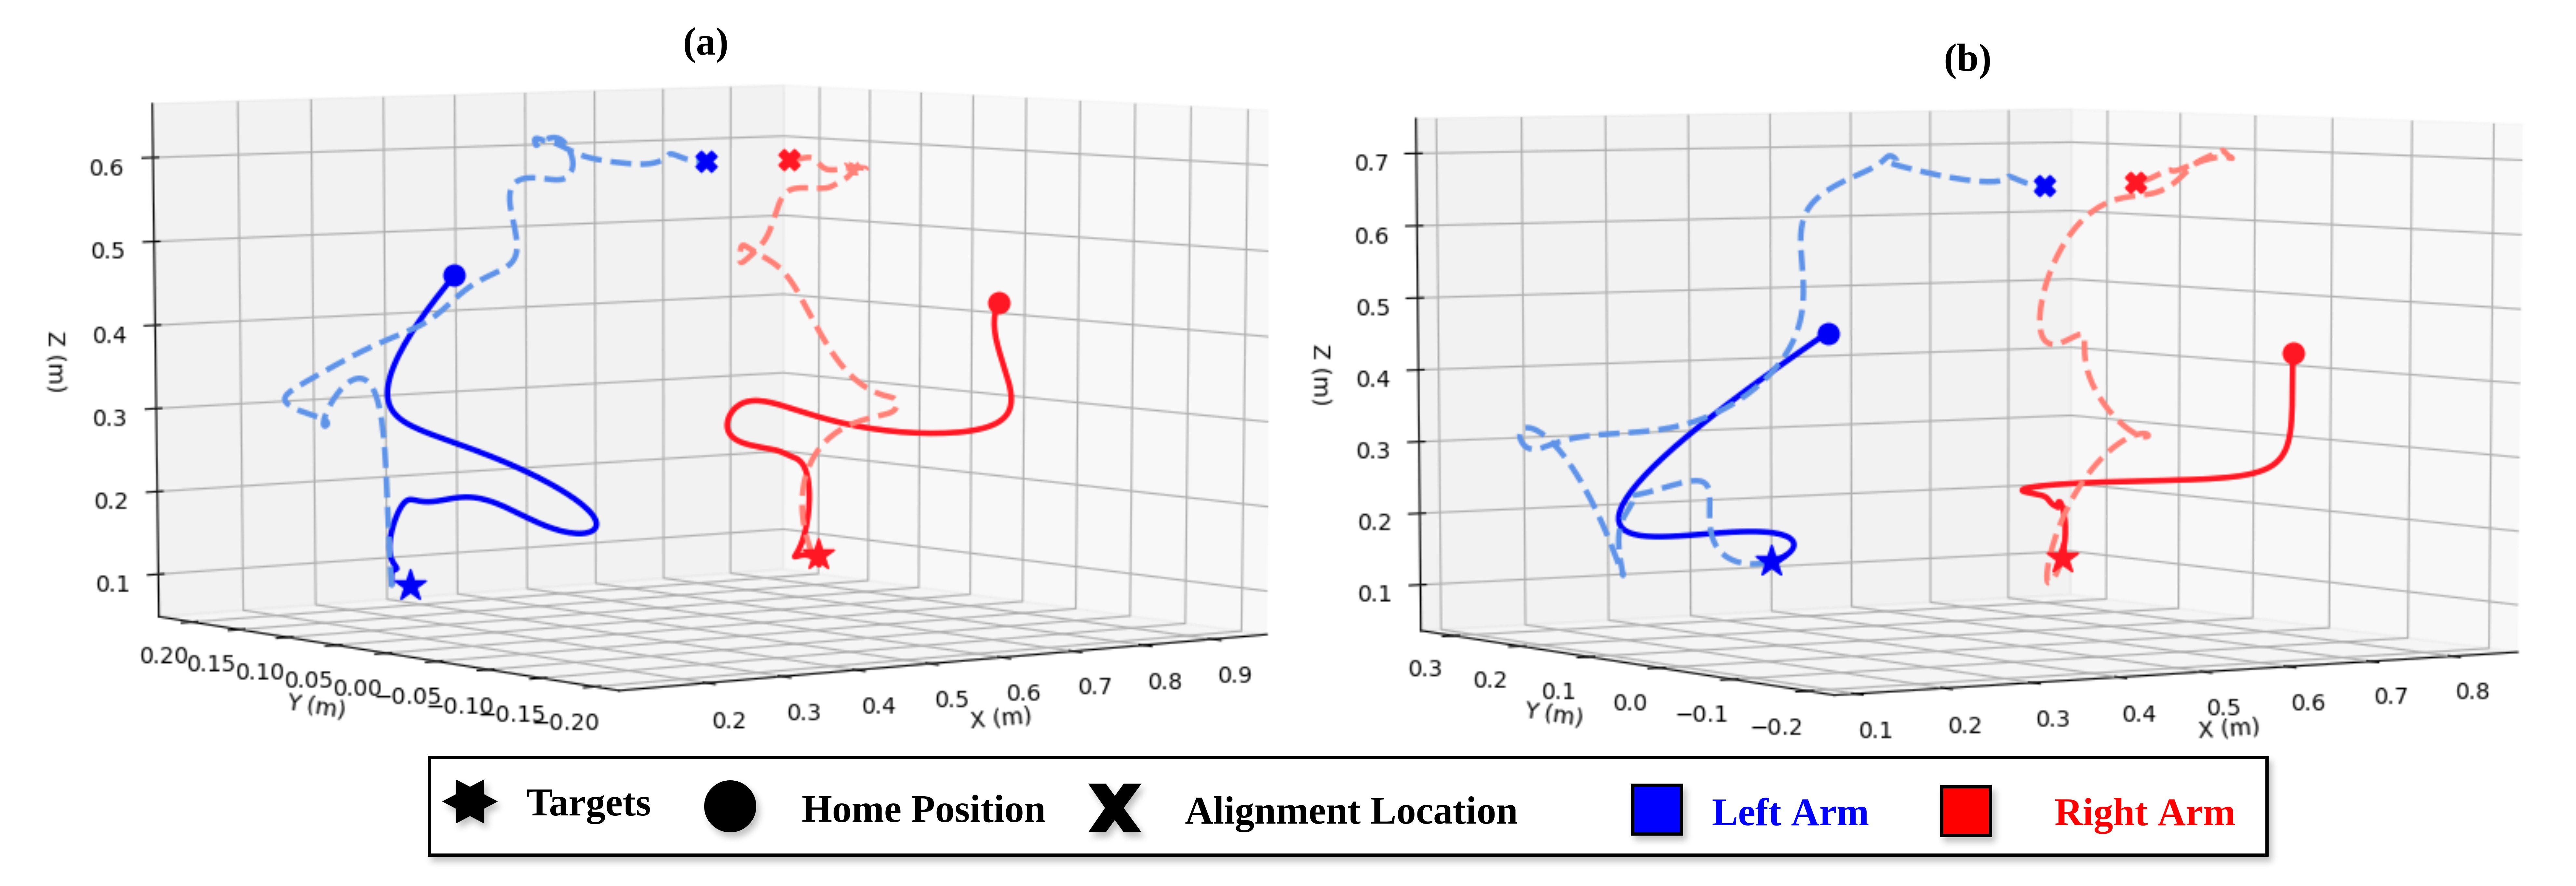
\includegraphics[width=0.85\linewidth]{Images/alpha/hardware_trajectories.jpg}
\caption{End-effector trajectories of the dual-arm system during the two real-hardware experiments: (a) Experiment 1 and (b) Experiment 2.}
\label{fig:alpha_hwtraj}
\end{figure}

Real-time hardware experiments used two Kinova Gen3 Lite manipulators for collaborative pick and
pre-assembly alignment of cylindrical (Figure~\ref{fig:alpha_exp1}) and square
(Figure~\ref{fig:alpha_exp2}) peg-and-hole configurations, with corresponding end-effector
trajectories in Figure~\ref{fig:alpha_hwtraj}. Both arms reach their independent targets by
$T=4$\,s, descend to grasp once positional and orientational thresholds converge in $X$ and $Y$
while maintaining a safe $Z$ offset by $T=15$\,s, grasp at $T=20$\,s, retreat to a safe spatial
clearance by $T=25$\,s, reach pre-docking positions by $T=52$\,s, and complete collaborative axial
alignment by $T=60$\,s.

\begin{table}[htbp]
\centering
\caption{Hardware deployment results over 30 trials with varied target positions~\citep{sk2025alpha}.}
\label{tab:alpha_hwresults}
\begin{tabular}{lccc}
\toprule
\textbf{Outcome} & \textbf{Reach} & \textbf{Align} & \textbf{Count} \\
\midrule
Successful execution            & \checkmark & \checkmark & 27 \\
Object slipped during insertion & \checkmark & $\times$   & 1 \\
Gripper fault during grasping   & $\times$   & $\times$   & 2 \\
\midrule
\textbf{Success rate} & \textbf{93.3\%} & \textbf{90.0\%} & \textbf{30} \\
\bottomrule
\end{tabular}
\end{table}

Table~\ref{tab:alpha_hwresults} reports 30 hardware trials with varied target positions: 27 complete
successfully, one fails only at final insertion due to an object slip after a successful reach and
grasp, and two fail during the grasp itself due to a gripper fault, giving 93.3\% reach success and
90.0\% overall alignment success (96.4\% alignment success conditioned on a successful reach). Since
the simulation-only snap mechanism of Equation~\eqref{eq:alpha_snap} is entirely absent from the
hardware deployment, this 90\% success confirms directly that the learned coordination behaviour
that produces reliable bilateral alignment is encoded in the trained policy weights, not in the
reward structure or snap mechanism used to train them, exactly the claim gap G7 required to be
demonstrated rather than assumed.

The two studies in this chapter close the thesis's progression from single-arm classical vision to
dual-arm reinforcement learning: Part I produces a trajectory-tracking controller for a single
non-spherical wrist that generalizes across arbitrary continuous geometries without retraining, and
Part II reuses that exact controller, frozen, as the low-level prior a multi-agent coordination
policy learns to blend with, rather than compete against, closing gap G7 without re-deriving the
reachability that Part I already solved. Chapter 9 concludes the thesis with a summary of
contributions across all eight studies, a discussion of the limitations each chapter has already
noted in its own scope, and directions for future work.
